% !TeX program = xelatex
\documentclass[runningheads]{llncs}
\usepackage[paperheight=295mm,paperwidth=210mm]{geometry}
\usepackage{graphicx}
\usepackage{wrapfig}
\usepackage{import}
\usepackage{kotex}
\usepackage[dvipsnames]{xcolor}
\usepackage{fancyvrb} %
\usepackage{listings}
\usepackage{tabularx}
\usepackage{underscore}
\usepackage{multicol}
\usepackage{enumitem}
\usepackage{subcaption}
\usepackage[numbers,square,super]{natbib}
\usepackage{mathptmx} % Times New Roman
\usepackage{amsmath}
\usepackage{amssymb}
\usepackage{framed}
\usepackage{etoolbox}
\usepackage{cancel}
\usepackage{physics}
\usepackage{tikz}
\usepackage{parskip}
\usepackage{enumerate}
\usepackage{minted}
\usepackage{inconsolata}
\usepackage{makecell}
\usepackage{slashed}
\usepackage{nicematrix}
\usetikzlibrary{calc, angles, quotes, graphs, positioning, arrows}

\setcounter{tocdepth}{2}

\colorlet{shadecolor}{gray!30}

\newcommand\enclosebox[2]{%
  \BeforeBeginEnvironment{#1}{\begin{#2}}%
  \AfterEndEnvironment{#1}{\end{#2}}%
}

\enclosebox{theorem}{oframed}
\enclosebox{definition}{leftbar}

\newcommand{\divides}{\bigm|}
\newcommand{\ndivides}{%
  \mathrel{\mkern.5mu % small adjustment
    % superimpose \nmid to \big|
    \ooalign{\hidewidth$\big|$\hidewidth\cr$\nmid$\cr}%
  }%
}
\newcommand{\ord}{\operatorname{\mathrm{ord}}}
\newcommand{\ind}{\operatorname{\mathrm{ind}}}
\newcommand{\legendre}[2]{\left(\frac{#1}{#2}\right)}
\setmainfont{Times New Roman}
\setmainhangulfont{Nanum Myeongjo}
\setmonofont{SF Mono}
\setlength{\parindent}{1em}
\setlength{\parskip}{0pt}
\linespread{1.2}
%\renewcommand{\arraystretch}{1.5}
\setlength{\tabcolsep}{0.5em}%
\newenvironment{Figure}
  {\par\medskip\noindent\minipage{\linewidth}}
  {\endminipage\par\medskip}
\newcommand{\translation}[1]{\textsuperscript{#1}}

\makeatletter
\renewcommand\NAT@citesuper[3]{\ifNAT@swa
\if*#2*\else#2\NAT@spacechar\fi
\unskip\kern\p@\textsuperscript{\NAT@@open#1\if*#3*\else,\NAT@spacechar#3\fi\NAT@@close}%
   \else #1\fi\endgroup}
\makeatother

\let\oldtabular\tabular% Store a copy of \tabular
\let\endoldtabular\endtabular% Store a copy of \endtabular
\renewenvironment{tabular}[2][\arraystretch]
  {\edef\arraystretch{#1}% Update \arraystretch
   \oldtabular{#2}}% \begin{tabular}[<stretch>]{<col spec>}
  {\endoldtabular}% \end{tabular}

\begin{document}

\title{Java Programming (0409)\newline\space Final Project Report}
\author{Department of Computer Science and Engineering, Konkuk University\newline\space Yulwon Rhee (202211342)}
\renewcommand\leftmark{Yulwon Rhee (202211342)}
\institute{담당 교수: 지정희 교수님\newline제출일: 2022년 12월 9일 금요일}

\maketitle
\section{문제 정의 및 분석}
본 프로젝트는 Java와 Swing을 이용하여 빙고 게임 데스크탑 애플리케이션을 제작하는 것을 목표로 한다.

\subsection{문제 정의}
\textbf{빙고판 생성:}
사용자에게 $N$\textsuperscript{빙고판의 크기}을 입력받은 후, 단어장 파일에서 $N^2$개의 랜덤한 단어를 골라 빙고판을 두 개 생성한다.

\textbf{턴 진행:}
빙고 게임은 유저와 컴퓨터가 번갈아가며 빙고판의 단어를 선택하는 식으로 진행한다.

\textbf{단어 선택:}
빙고판의 단어가 선택된 경우, 선택된 단어와 그 단어의 뜻을 출력한다.

\textbf{단어 체크:}
유저와 컴퓨터의 빙고판에 선택된 단어가 있는지 확인하고, 체크한다.

\textbf{컴퓨터의 단어 선택:}
컴퓨터가 단어를 선택할 때에는 승리를 위한 알고리즘을 설계하여 그에 따라 선택하도록 한다.

\textbf{빙고 체크:}
한 턴이 진행된 후마다 빙고 수를 체크한다. 빙고의 수가 1개 이상 많은 경우 승리하도록 한다.

\textbf{승률 저장:}
사용자와 컴퓨터의 승률을 파일로 저장하여, 다음 실행 시에도 불러오도록 한다.

\textbf{UI 개선:}
Swing을 이용하여 UI를 개선한다.

\newpage
\section{주요 소스코드 설명}
메소드들은 여러 클래스에 나뉘어 존재한다.

\begin{tabularx}{\textwidth}{l|X}
    \hline
    파일 이름                         & 역할                                  \\
    \hline
    \texttt{BingoGame.java}       & 프로그램의 시작점. 상황에 맞는 Frame을 띄워준다.      \\
    \hline
    \texttt{Game.java}            & 통계를 위한 게임 정보를 관리하는 Class.           \\
    \texttt{User.java}            & 플레이어와 컴퓨터의 게임 중 데이터를 관리하는 Class.    \\
    \texttt{Word.java}            & 단어장에서 단어를 불러오고, 이를 관리하는 Class.      \\
    \hline
    \texttt{StatisticUtil.java}   & 통계를 관리하는 Class.                     \\
    \hline
    \texttt{StartFrame.java}      & 게임을 시작하기 전 필요한 정보를 수집하는 Frame.      \\
    \texttt{GameFrame.java}       & 게임 화면 Frame. 게임과 관련된 동작이 여기서 이루어진다. \\
    \texttt{StatisticDialog.java} & 통계를 자세히 보여주는 Dialog.                \\
    \hline
\end{tabularx}

\subsection{\texttt{BingoGame.java}}
\mintinline{java}{public static void main(String[] args)}:
프로그램의 시작점으로써,
시작 시 저장된 통계 파일을 읽어와 \mintinline{java}{StartFrame}을 호출한다.
이후, \mintinline{java}{StartFrame}에서 단어장 파일, $N$의 값과 AI 수준을 받아와 \mintinline{java}{GameFrame}을 호출한다.
게임이 끝나면, 게임 시작 시간, $N$의 값, AI 수준과 승패 여부를 받아와 통계 리스트에 저장하고, 통계 파일에 추가한다.

\subsubsection{Source Code}
\inputminted[fontsize=\scriptsize]{java}{../../src/main/java/ywrhee/project/BingoGame.java}

\newpage
\subsection{\texttt{Game.java}}
승패 여부, $N$의 값, AI 수준 및 게임 플레이 시간 등 게임 데이터를 관리하는 Class이다.
게임에 필요한 상수가 \mintinline{java}{static}으로 선언되어 있고, 통계 파일에서 데이터를 파싱해 \mintinline{java}{Game} 클래스로 바꿔주는 \mintinline{java}{static} 메소드가 포함되어 있다.

\mintinline{java}{public String getCsvInfo()}:
게임 데이터를 CSV\textsuperscript{Comma-Seperated Values} 형태로 변환해 텍스트 형태로 저장하기 쉽게 반환한다.

\mintinline{java}{public Object[] getTableRow(int winLoseInfo)}:
게임 데이터를 \mintinline{java}{JTable}의 Row에 바로 넣을 수 있도록 가공하여 반환한다.

\mintinline{java}{public static Game parseGameInfo(String gameInfoAsCsv)}:
CSV 형태로 변환된 게임 데이터를 파싱하여 다시 \mintinline{java}{Game} 객체로 되돌려 반환한다.
인스턴스를 생성하지 않아도 바로 쓸 수 있게 \mintinline{java}{static} 메소드로 만들었다.

\subsubsection{Source Code}
\inputminted[fontsize=\scriptsize]{java}{../../src/main/java/ywrhee/project/Game.java}

\newpage
\subsection{\texttt{User.java}}
유저 및 컴퓨터의 빙고판, 빙고 갯수, 단어 목록 등을 묶어 편하게 관리하기 위한 Class이다.

\mintinline{java}{public User(ArrayList<Word> fullWordList, int N)}:
\mintinline{java}{User} 클래스의 생성자로써,\\\mintinline{java}{fullWordList}\textsuperscript{단어장에서 받아온 전체 단어 리스트}와 $N$을 파라미터로 받아 $N^2$ 크기의 빙고판을 만든다.
\mintinline{java}{Collections.shuffle()} 메소드를 이용하여 \mintinline{java}{fullWordList}를 랜덤하게 섞어 맨 앞 $N^2$개의 단어를 선택하는 방식으로 해당 기능을 구현했다.

\mintinline{java}{public void constructBingoPanel()}:
Swing의 \mintinline{java}{GridLayout}을 사용하여 빙고판 레이아웃을 만든다. 빙고판을 다시 그릴 때마다 호출된다.

\mintinline{java}{public boolean isSelectable()}:
플레이어의 빙고판에 선택할 수 있는 단어가 남았는지 여부를 반환한다.

\mintinline{java}{public void updateBingoCount()}:
플레이어의 빙고판에서 빙고의 갯수를 계산한다.

\mintinline{java}{public Word selectWordToWin(int difficulty, ArrayList<Word> comparableList)}:
컴퓨터가 사용하는 메소드로써, 이기기 위해 선택해야 할 단어를 반환한다. 컴퓨터가 단어를 선택하는 알고리즘은 다음과 같다.\\\\
\begin{tabularx}{\textwidth}{l|X}
    \hline
    난이도 & 선택 알고리즘                                                \\
    \hline
    쉬움  & 컴퓨터의 빙고판에서 선택되지 않은 단어 중 하나를 랜덤으로 뽑아 반환한다.              \\
    % \hline
    중간  & 가로, 세로, 대각선 중 가장 빙고에 가까운 줄에서 선택되지 않은 단어를 골라 반환한다.      \\
    % \hline
    어려움 & 만약 $N$이 홀수이고, 가장 처음 선택되는 단어일 경우 빙고판 한가운데를 먼저 선택해 반환한다.
    $N$이 홀수가 아니거나 가장 처음 선택되는 단어가 아니라면 가로, 세로, 대각선 중 가장 빙고에 가까운 줄에서 선택되지 않은 단어를 반환하되,
    $1/2$의 확률로 사용자의 빙고판에 없는 단어를 우선적으로 골라 반환한다.
    만약 사용자의 빙고판에 있는 단어더라도, 그 단어만 선택하면 빙고가 완성될 경우, 그 단어를 반환한다.    \\
    \hline
\end{tabularx}

\subsubsection{Source Code}
\inputminted[fontsize=\scriptsize]{java}{../../src/main/java/ywrhee/project/User.java}

\newpage
\subsection{\texttt{Word.java}}
단어의 영어, 한국어 뜻, 빙고판에서 선택 여부, 이 단어를 선택했을 경우 빙고가 될 확률을 묶어 편하게 관리하기 위한 Class이다.
단어장 파일에서 단어를 읽어오는 \mintinline{java}{static} 메소드가 포함되어 있다.

\mintinline{java}{public static ArrayList<Word> getWordList(File file)}:
단어장 파일에서 영단어와 한국어 뜻을 읽어와 \mintinline{java}{Word} 클래스 형태로 바꾸어 리스트에 넣어 반환한다.
인스턴스를 생성하지 않아도 바로 쓸 수 있게 \mintinline{java}{static} 메소드로 만들었다.

\subsubsection{Source Code}
\inputminted[fontsize=\scriptsize]{java}{../../src/main/java/ywrhee/project/Word.java}

\newpage
\subsection{\texttt{StatisticUtil.java}}
통계를 편리하게 관리하기 위한 유틸리티 Class이다.
인스턴스를 생성하지 않아도 바로 쓸 수 있게 모두 \mintinline{java}{static} 메소드로 만들었다.

\mintinline{java}{public static void init()}:
CSV 형식으로 쓰여진 통계 파일에서 통계를 파싱해 \mintinline{java}{statisticList}에 저장하고,
통계 정보를 기록할 수 있는 \mintinline{java}{FileWriter}를 초기화한다.

\mintinline{java}{public static void addToStatisticList(Game game)}:
게임 데이터를 \mintinline{java}{statisticList}에 저장한다.

\mintinline{java}{public static void writeStatistic(Game game)}:
CSV 형식으로 변환된 게임 데이터를 \mintinline{java}{FileWriter}로 이어쓴 후, 버퍼를 Flush한다.

\mintinline{java}{public static void closeStatisticWriterStream()}:
\mintinline{java}{FileWriter}의 \mintinline{java}{InputStream}을 \mintinline{java}{close}한다.

\subsubsection{Source Code}
\inputminted[fontsize=\scriptsize]{java}{../../src/main/java/ywrhee/project/StatisticUtil.java}

\newpage
\subsection{\texttt{StartFrame.java}}
게임을 시작하기 전 필요한 정보인 단어장 파일, AI 수준, $N$을 입력받고, 저장된 통계 정보를 출력하는 Frame이다.

\mintinline{java}{public StartFrame(String title, ArrayList<Game> statisticList)}:
\mintinline{java}{StartFrame}의 생성자로써, 윈도우의 타이틀과 통계 목록을 파라미터로 받아 클래스 내에서 사용 가능하도록 한다.
게임을 시작하기 위해 필요한 정보가 입력될 때까지 메인 스레드에서 입력 받은 값을 접근할 수 없도록 \mintinline{java}{this.wait()}을 사용한다.

\mintinline{java}{private void initUI()}:
게임에 필요한 정보를 수집할 UI를 구성한다.
생성자를 통해 넘겨받은 통계 정보를 이용해 화면에 승률을 표시하고, 클릭 시 \mintinline{java}{StatisticDialog}가 호출되도록 한다.

\mintinline{java}{public void actionPerformed(ActionEvent e)}:
\mintinline{java}{ActionListener}의 \mintinline{java}{actionPerformed}를 Override한 메소드로,
시작하기 버튼이 눌렸거나 $N$을 입력받는 텍스트 필드에서 Enter 키가 눌렸을 때 호출된다.
선택된 단어장 파일의 존재 여부와, $N$값의 유효성(단어장의 단어 갯수가 $N^2$ 보다 큰지, $3 \leq N \leq 10$인지)을 체크하여 정상적인 실행이 불가할 경우 경고 Dialog를 띄운다.
만약 정상적으로 게임이 실행 가능하면 메인 스레드에서 \mintinline{java}{GameFrame}을 호출할 수 있도록 \mintinline{java}{this.notify()}해주고 윈도우를 \mintinline{java}{dispose()}한다.

\mintinline{java}{private int countLine(File file)}:
파라미터로 전달받은 단어장 파일의 단어 갯수를 반환한다.

\subsubsection{Source Code}
\inputminted[fontsize=\scriptsize]{java}{../../src/main/java/ywrhee/project/StartFrame.java}

\newpage
\subsection{\texttt{GameFrame.java}}
게임 화면을 출력하는 Frame이다.

\mintinline{java}{public GameFrame(String title, User user, User computer, int N, int difficulty)}:
\mintinline{java}{GameFrame}의 생성자로써, 윈도우 타이틀, 유저 및 컴퓨터의 플레이 데이터, $N$값과 AI 수준을 파라미터로 입력받아 Class 내에서 사용 가능하도록 한다.
게임 데이터가 완성될 때까지 메인 스레드에서 \mintinline{java}{GameFrame}의 데이터를 접근할 수 없도록 \mintinline{java}{this.wait()}을 사용한다.

\mintinline{java}{private void initUI()}:
게임 플레이 UI를 구성한다.

\mintinline{java}{public void actionPerformed(ActionEvent e)}:
\mintinline{java}{ActionListener}의 \mintinline{java}{actionPerformed}를 Override한 메소드로,
단어 입력 버튼이 눌렸거나 단어를 입력받는 텍스트 필드에서 Enter키가 눌렸을 때 호출된다.
만약 입력받은 단어가 컴퓨터 또는 유저의 빙고판에 존재할 경우, 체크해주고 빙고판을 다시 그리도록 \mintinline{java}{updateBingoBoard()}를 호출하고, 선택된 단어의 뜻을 출력한다.
이후 \mintinline{java}{computerTurn()}이 호출되어 컴퓨터의 턴으로 넘어간다.

\mintinline{java}{private void computerTurn()}:
컴퓨터의 빙고판에 선택 가능한 단어가 남아있을 경우,
\mintinline{java}{User} 클래스의 \mintinline{java}{selectWordToWin()} 메소드를 이용하여 단어를 선택한다.
바로 선택하여 유저 턴으로 넘어가는 모습이 어색하지 않도록 1000ms의 딜레이 이후에 컴퓨터가 선택한 단어가 출력되고, 빙고판을 다시 그리도록 \mintinline{java}{updateBingoBoard()}를 호출한다.
이후 승패 여부를 가리도록 \mintinline{java}{checkWinner()} 메소드를 호출한다.

\mintinline{java}{private void checkWinner()}:
한 턴이 끝난 후 호출되는 메소드로써, 유저와 컴퓨터의 빙고판을 체크하여 빙고의 갯수가 한 개이상 많은 플레이어를 승리로 처리한다.
빙고판이 모두 열렸지만 승패가 결정되지 않은 경우 무승부로 처리한다.
이후 결정된 승패 정보를 Dialog로 출력하고, 게임 화면을 종료하도록 \mintinline{java}{closeGameFrame()}을 호출한다.

\mintinline{java}{private void updateBingoBoard()}:
유저와 컴퓨터의 빙고판에 선택된 단어를 표시하여 다시 그린다.

\mintinline{java}{private void closeGameFrame()}:
메인 스레드에서 \mintinline{java}{GameFrame}의 데이터를 접근할 수 있도록 \mintinline{java}{this.notify()}하고 윈도우를 \mintinline{java}{dispose()}한다.

\subsubsection{Source Code}
\inputminted[fontsize=\scriptsize]{java}{../../src/main/java/ywrhee/project/GameFrame.java}

\newpage
\subsection{\texttt{StatisticDialog.java}}
통계 정보를 테이블로 출력하는 Dialog이다.

\mintinline{java}{public StatisticDialog(StartFrame owner, String title, ArrayList<Game> statisticList, String statisticInfo)}:
\mintinline{java}{StatisticDialog}의 생성자로써, 부모 Frame, 윈도우 타이틀, 통계 데이터를 파라미터로 입력받아 Class 내에서 사용 가능하도록 한다.

\mintinline{java}{private void initUI()}:
통계 화면 UI를 구성한다.
통계 데이터를 \mintinline{java}{JTable}에 표시하고, 승패 여부에 따라 Row의 배경 색을 바꾼다.

\subsubsection{Source Code}
\inputminted[fontsize=\scriptsize]{java}{../../src/main/java/ywrhee/project/StatisticDialog.java}

\newpage
\section{실행 결과}
\subsection{게임 전 화면}
\begin{figure}[h]
    \centering
    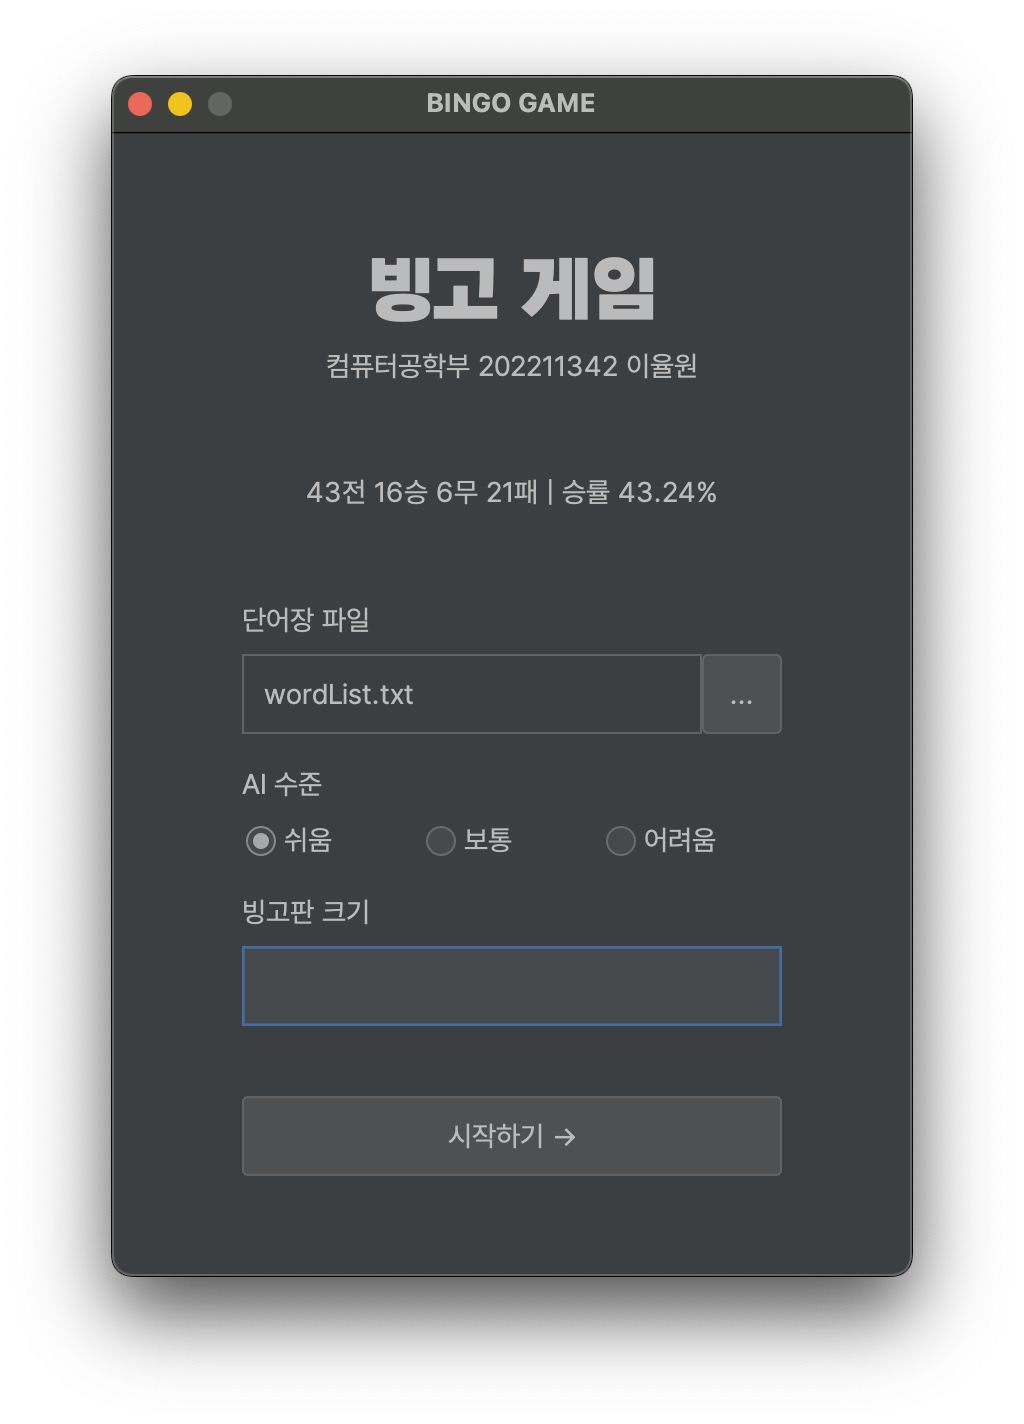
\includegraphics[scale=0.5]{img/main.png}
    \caption{메인 화면}
\end{figure}
이 화면에서는 게임 플레이 전 필요한 정보를 수집하는 역할을 한다.
화면 상단의 승률 Label을 클릭해 전체 통계를 볼 수 있고, 단어장 파일은 `...'이 적힌 버튼을 눌러 선택할 수 있다.
정보를 다 선택한 이후 엔터를 누르거나 `시작하기 →' 버튼을 눌러 게임 화면에 진입할 수 있다.
만약 선택된 파일이 없는 파일이거나, 입력된 $N$의 값이 $3 \leq N \leq 10$이 아닌 경우 경고창을 띄워주고,
단어장의 단어가 모자라 빙고판을 생성할 수 없는 경우,
입력받은 $N$ 값으로 빙고판을 생성하기 위해 필요한 최소 단어 수와, 선택된 단어장으로 생성 가능한 최대 $N$을 알려준다.
\newpage

\begin{figure}[H]
    \begin{subfigure}{.5\textwidth}
        \centering
        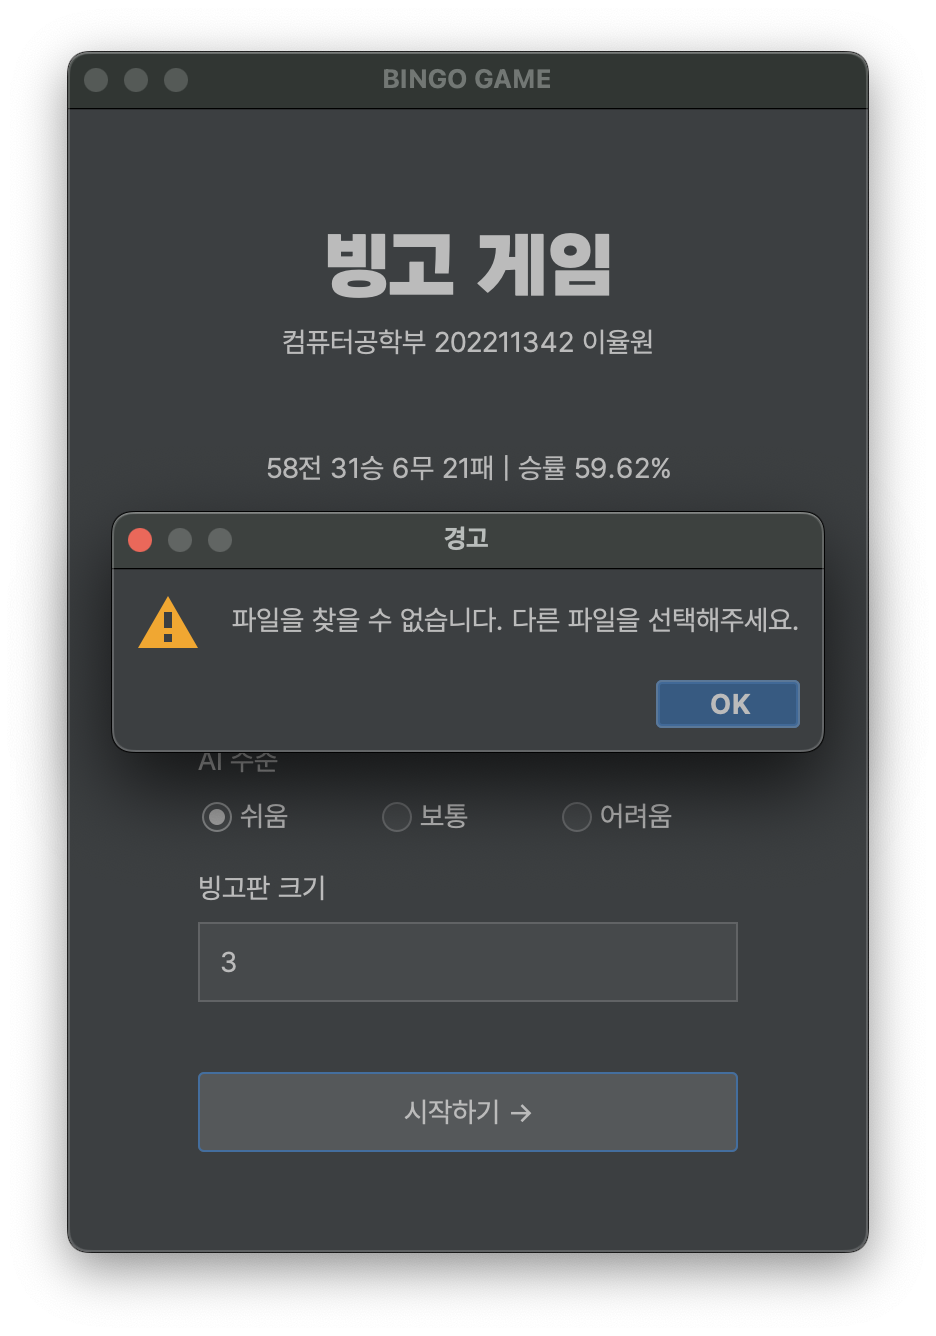
\includegraphics[scale=0.4]{img/main-file-not-found.png}
        \caption{선택된 파일이 없는 경우}
    \end{subfigure}
    \begin{subfigure}{.5\textwidth}
        \centering
        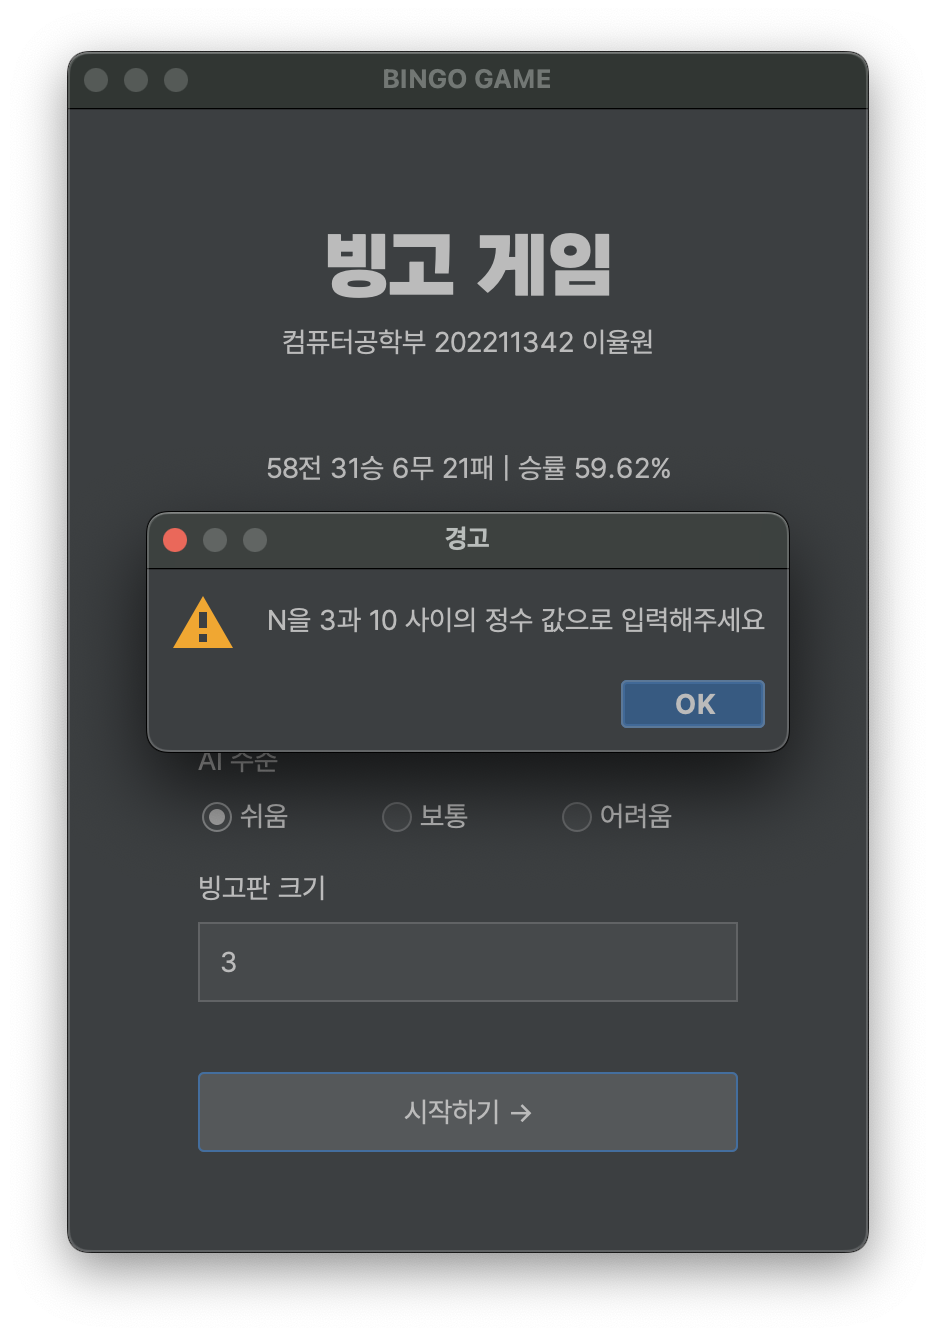
\includegraphics[scale=0.4]{img/main-n-range-error.png}
        \caption{$3 \leq N \leq 10$이 아닌 경우}
    \end{subfigure}
    \begin{subfigure}{\textwidth}
        \centering
        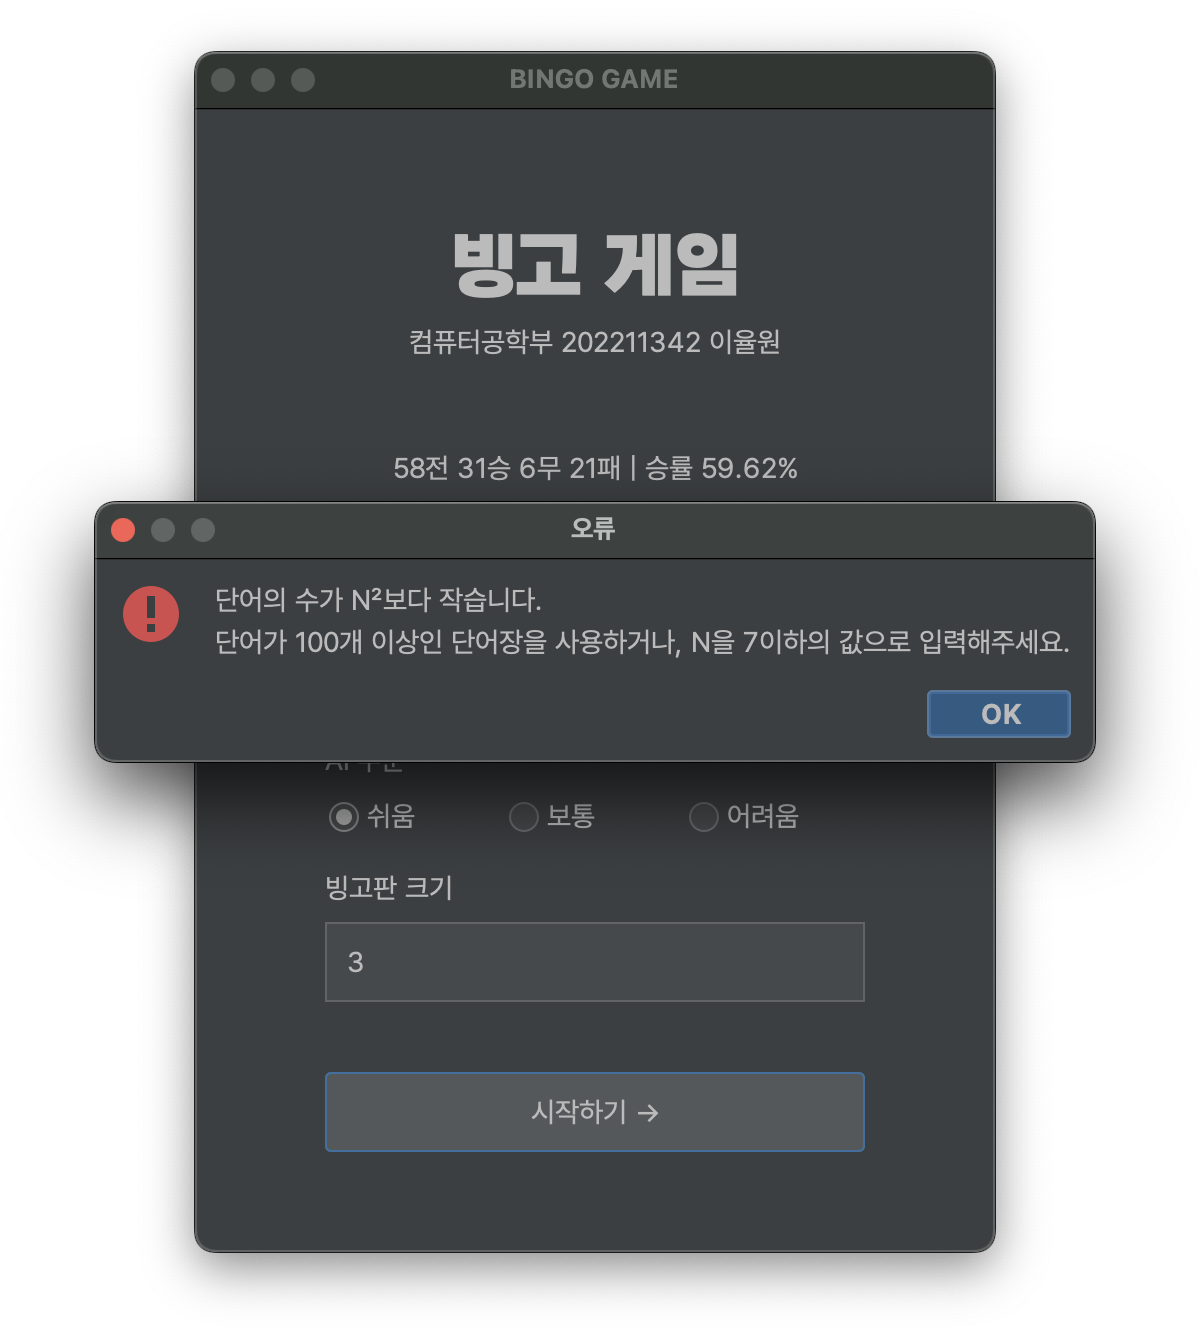
\includegraphics[scale=0.4]{img/main-word-list-size-error.png}
        \caption{$N = 10$일 때, 단어장의 단어가 모자라 빙고판을 생성할 수 없는 경우}
    \end{subfigure}
    \caption{사용자 입력 예외 처리}
\end{figure}

\begin{figure}[H]
    \centering
    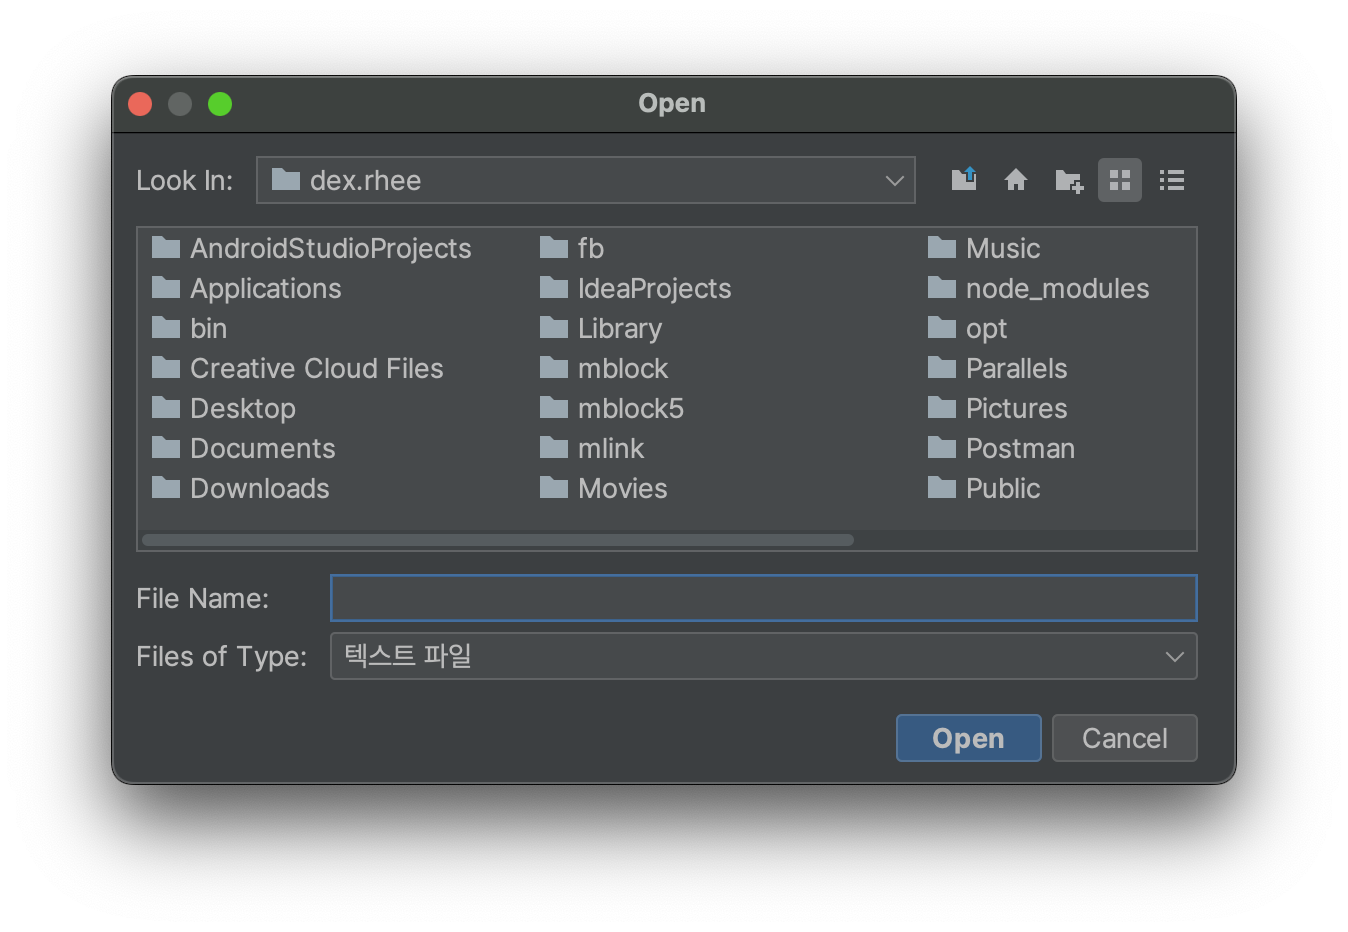
\includegraphics[scale=0.35]{img/file-chooser.png}
    \caption{단어장 파일 선택 Dialog}
\end{figure}
단어장 파일을 선택할 수 있다.
\texttt{JFileChooser}를 사용하여 구현하였다.

\begin{figure}[H]
    \centering
    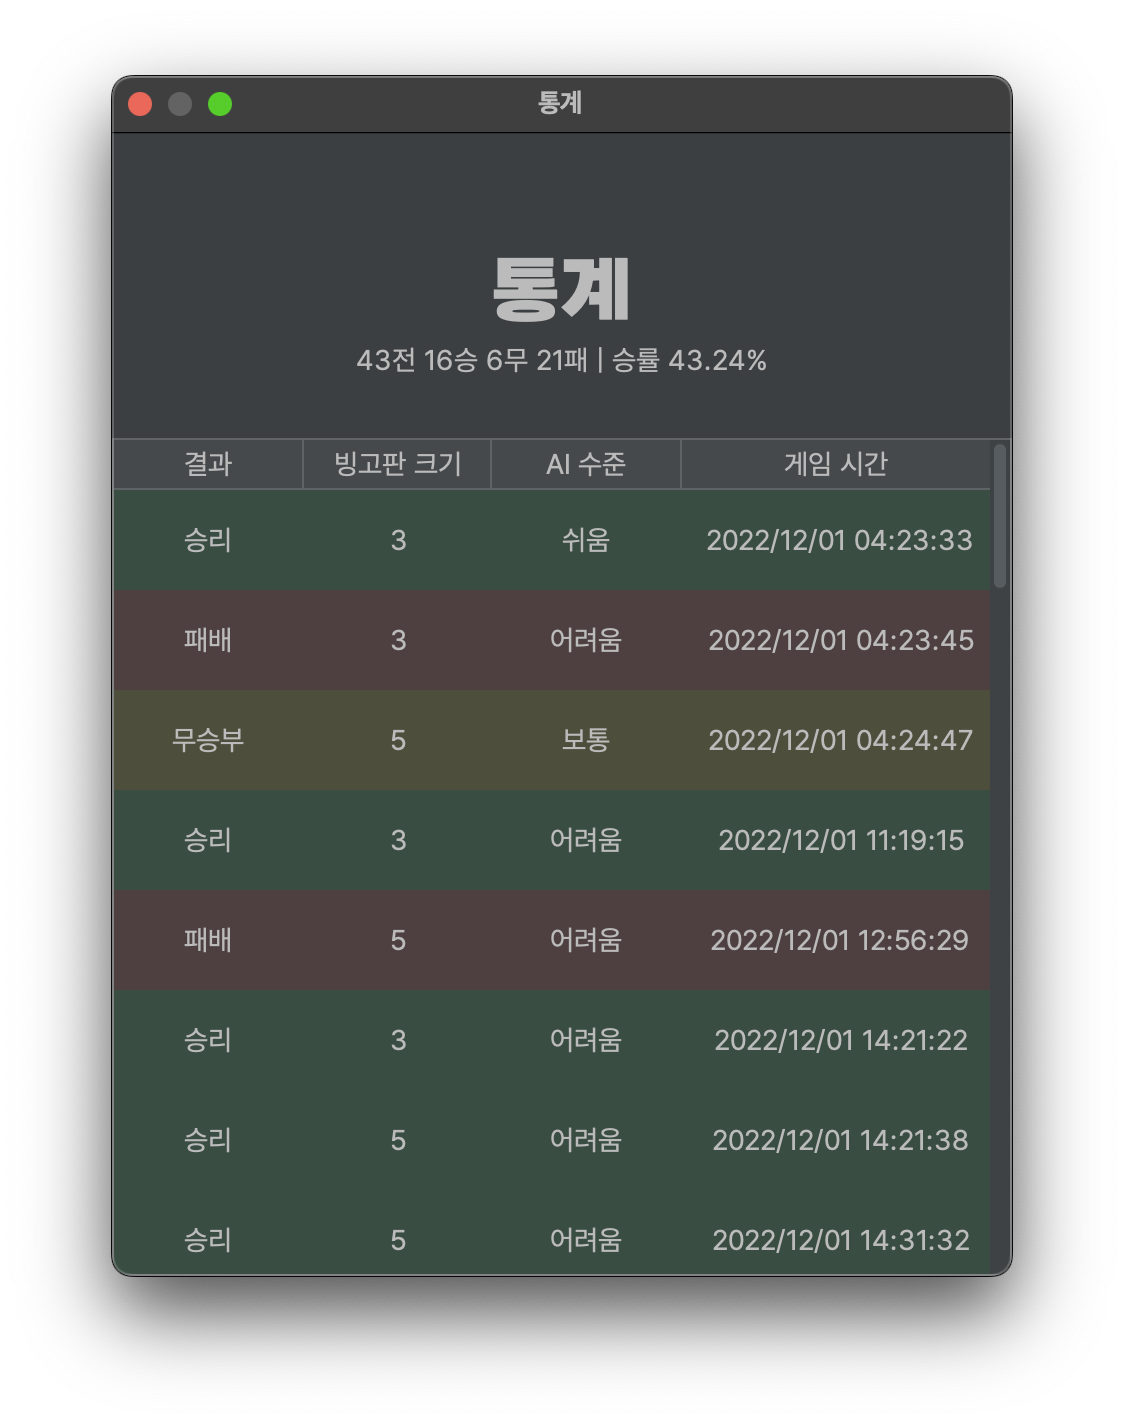
\includegraphics[scale=0.35]{img/statistic.png}
    \caption{통계 Dialog}
\end{figure}
이 Dialog에서는 플레이한 모든 게임의 승패 여부, 빙고판 크기, AI 수준, 게임 시간을 볼 수 있다.
Modal Dialog이기 때문에, 닫기 전까지 게임을 시작할 수 없다.

\newpage
\subsection{게임 중 화면}
\begin{figure}[H]
    \centering
    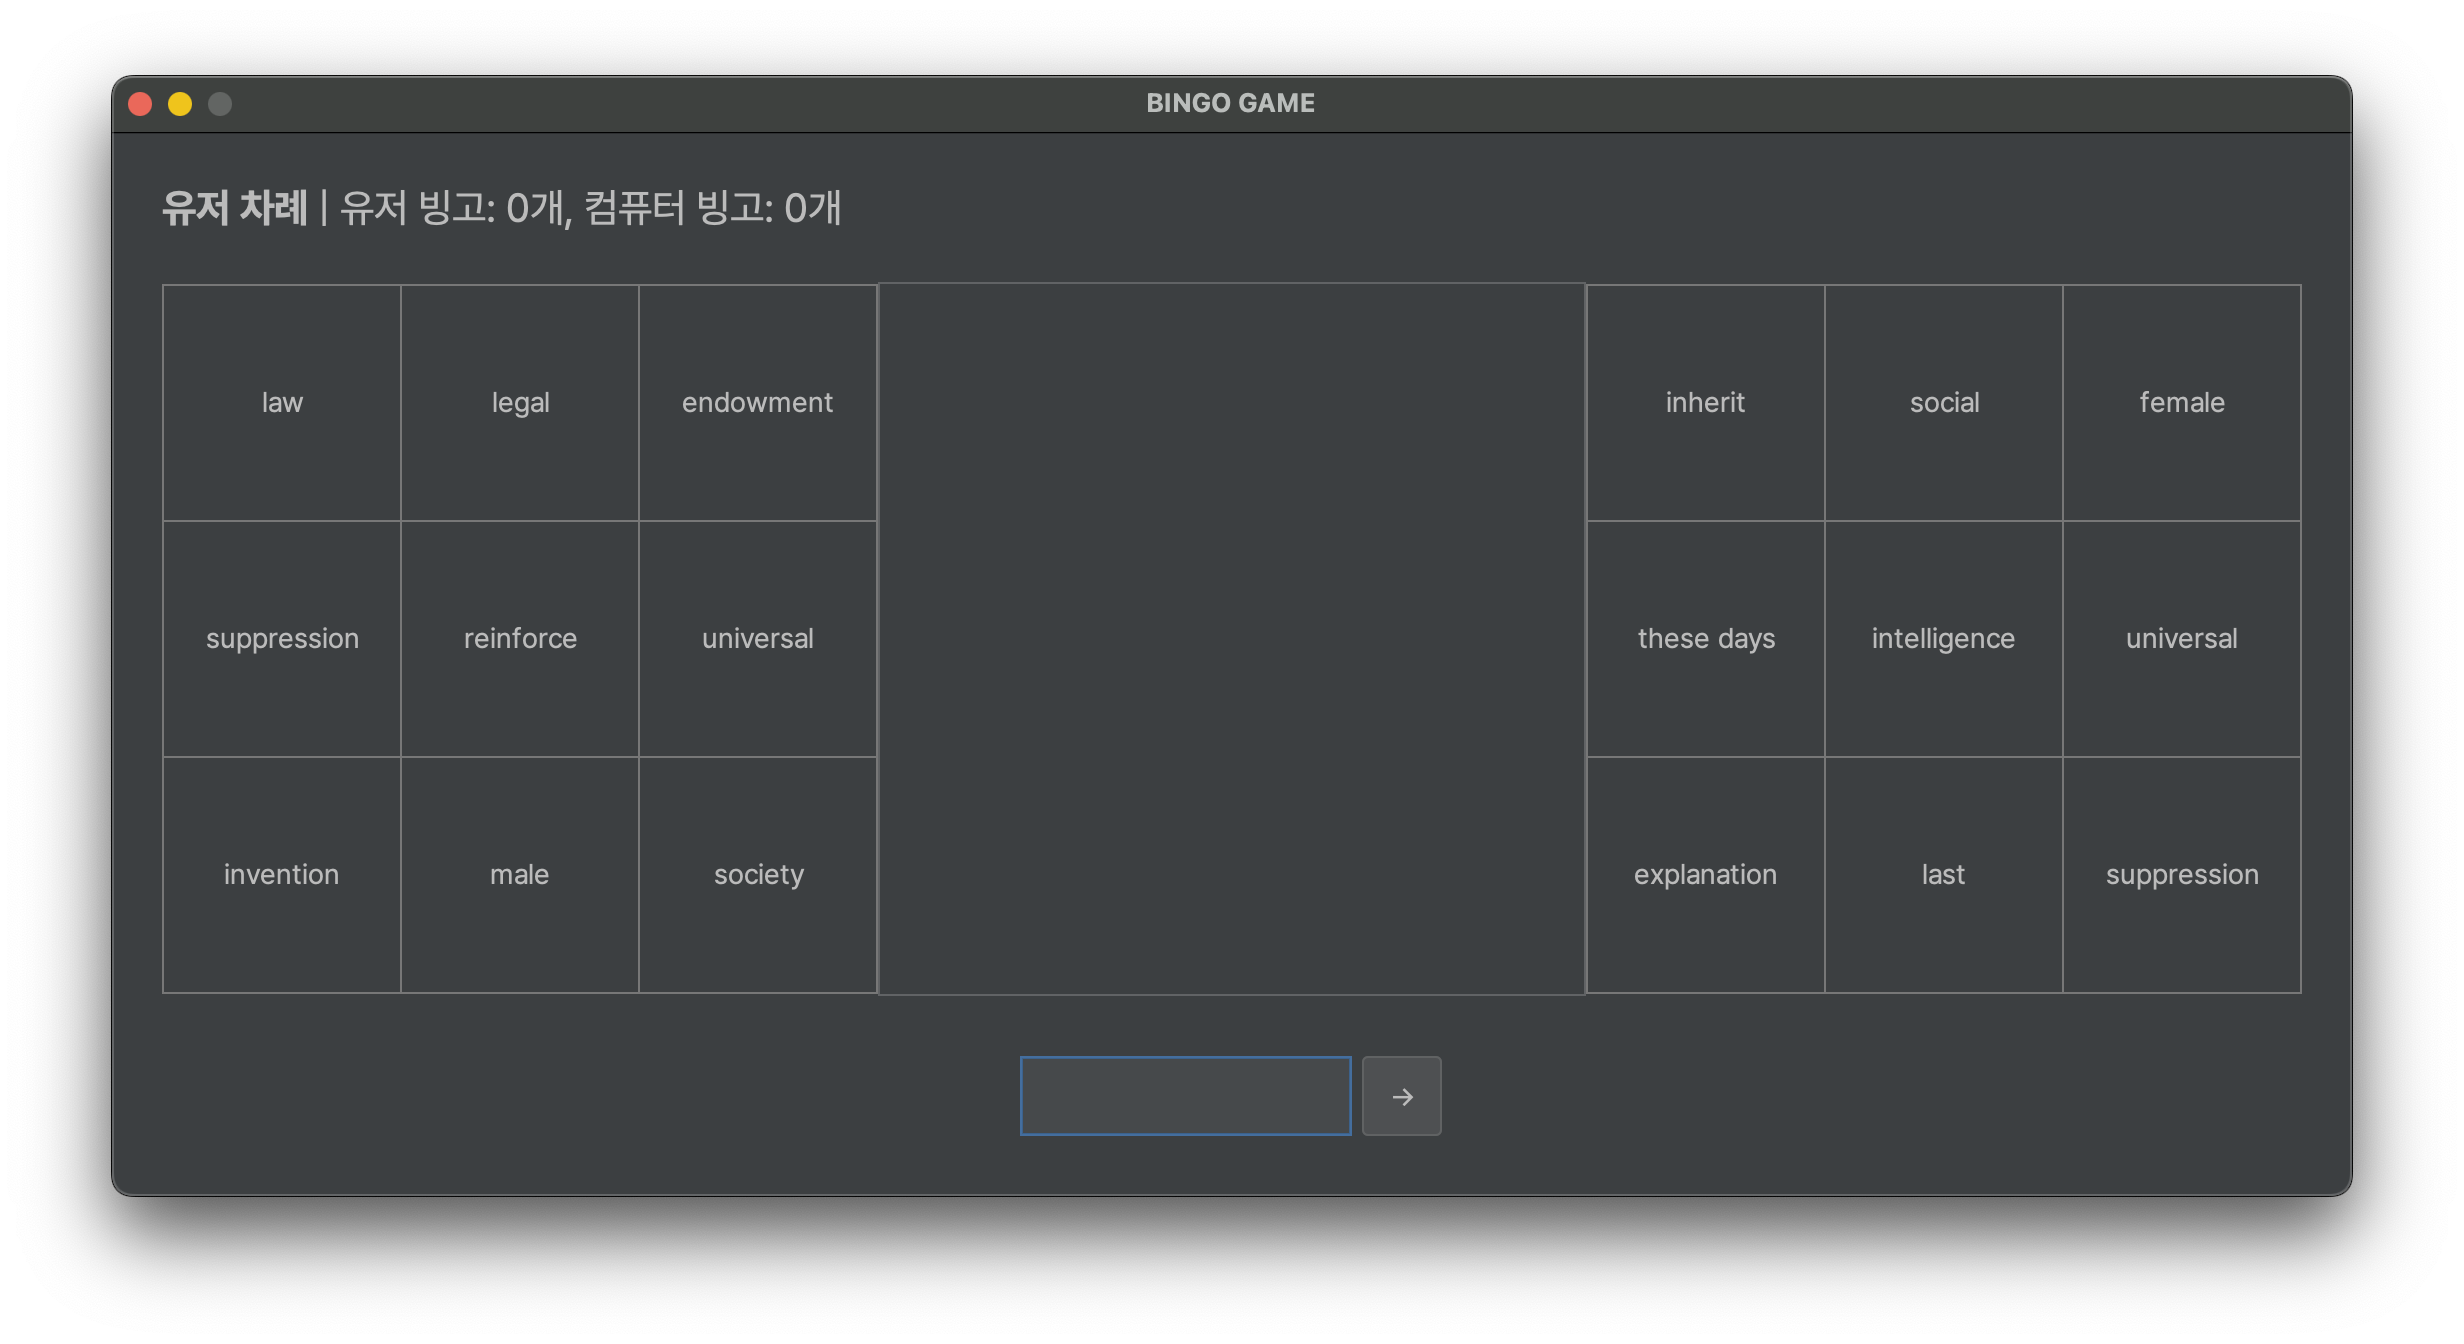
\includegraphics[scale=0.3]{img/game-3x3.png}
    \caption{$N = 3$일 때}
\end{figure}
$N$ 값을 3으로 입력했을 때 구성된 게임 화면이다.
유저 차례일 경우 아래의 텍스트 필드 및 버튼이 Enable 되고, 원하는 단어를 입력 후 Enter키를 누르거나, `→' 버튼을 눌러 선택할 수 있다.
컴퓨터 차례일 경우 아래의 텍스트 필드 및 버튼이 Disable 되고, 1초 후 컴퓨터가 선택한 단어가 화면에 표시된다.

\begin{figure}[H]
    \centering
    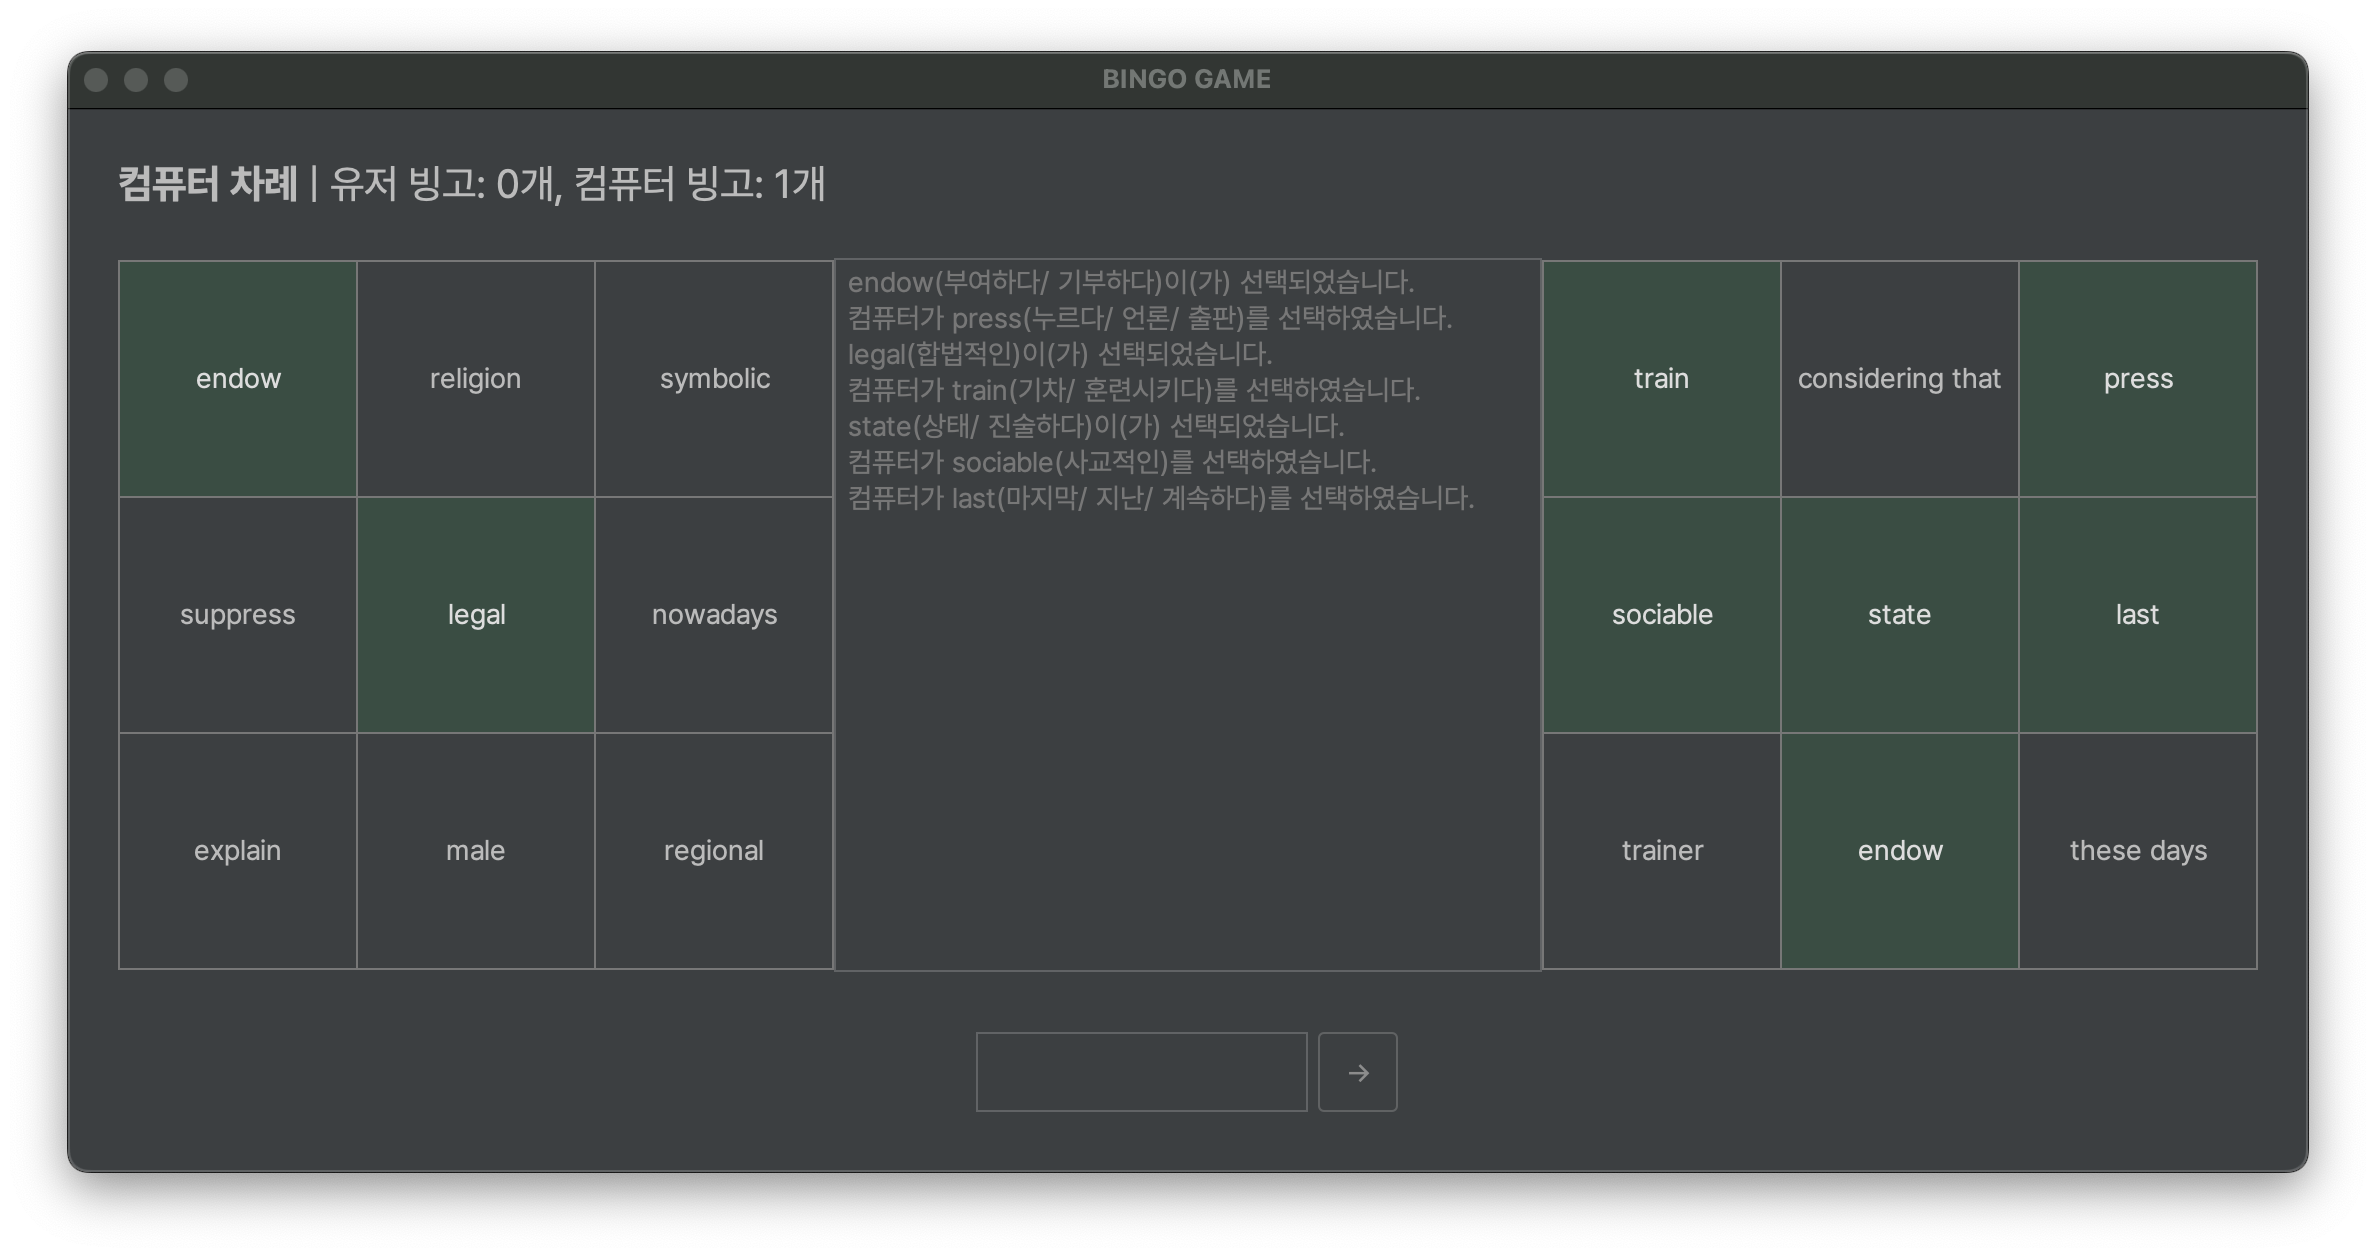
\includegraphics[scale=0.3]{img/game-3x3-playing.png}
    \caption{$N = 3$일 때 플레이 중 화면}
\end{figure}
유저가 선택한 단어가 유저 또는 컴퓨터의 빙고판에 존재할 경우, 해당 단어가 있는 빙고칸의 배경이 초록색으로 바뀌고(이하 체크), 선택한 단어와 단어의 뜻이 출력된다.
컴퓨터가 단어를 선택한 경우, 유저의 빙고판에 있는 동일한 단어도 체크된다.
만약 유저가 빙고판에 없는 단어를 입력했을 경우, 바로 컴퓨터의 턴으로 넘어간다.
만약 유저가 입력한 단어가 유저의 빙고판에는 없지만 컴퓨터의 빙고판에는 존재할 경우, 컴퓨터의 빙고판에 있는 해당 단어가 체크된다.
한 턴이 끝날 때마다 빙고 여부를 체크하고, 빙고 개수가 하나 이상 많은 플레이어를 승리 처리한다.

\begin{figure}[H]
    \begin{subfigure}{\textwidth}
        \centering
        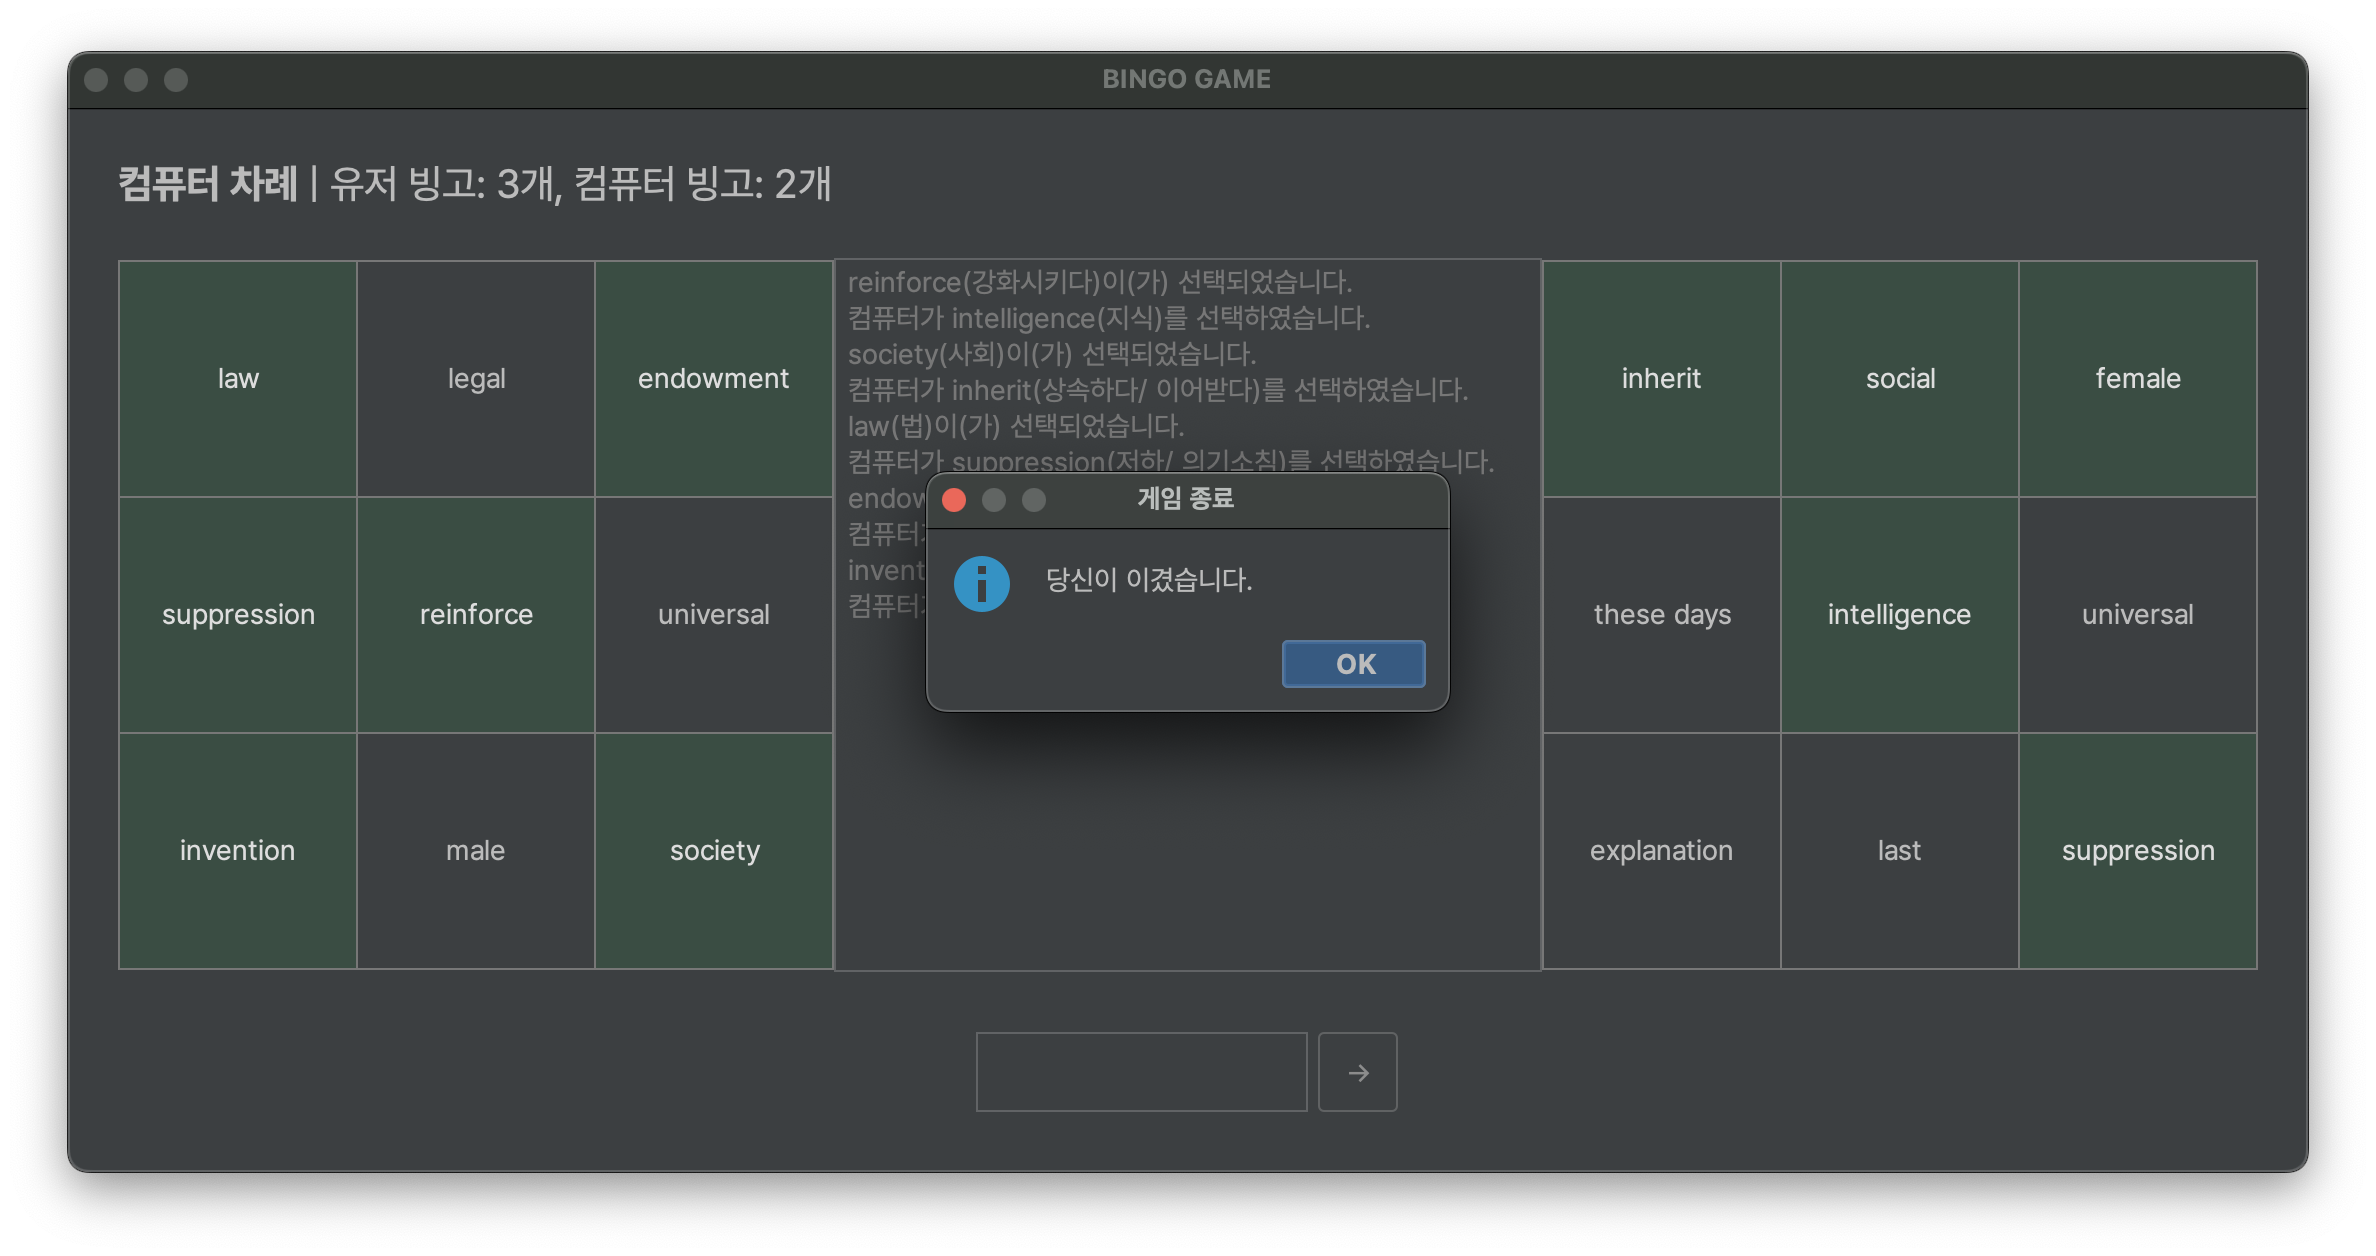
\includegraphics[scale=0.3]{img/game-3x3-victory.png}
        \caption{이겼을 때}
    \end{subfigure}
    \\\\\\
    \begin{subfigure}{\textwidth}
        \centering
        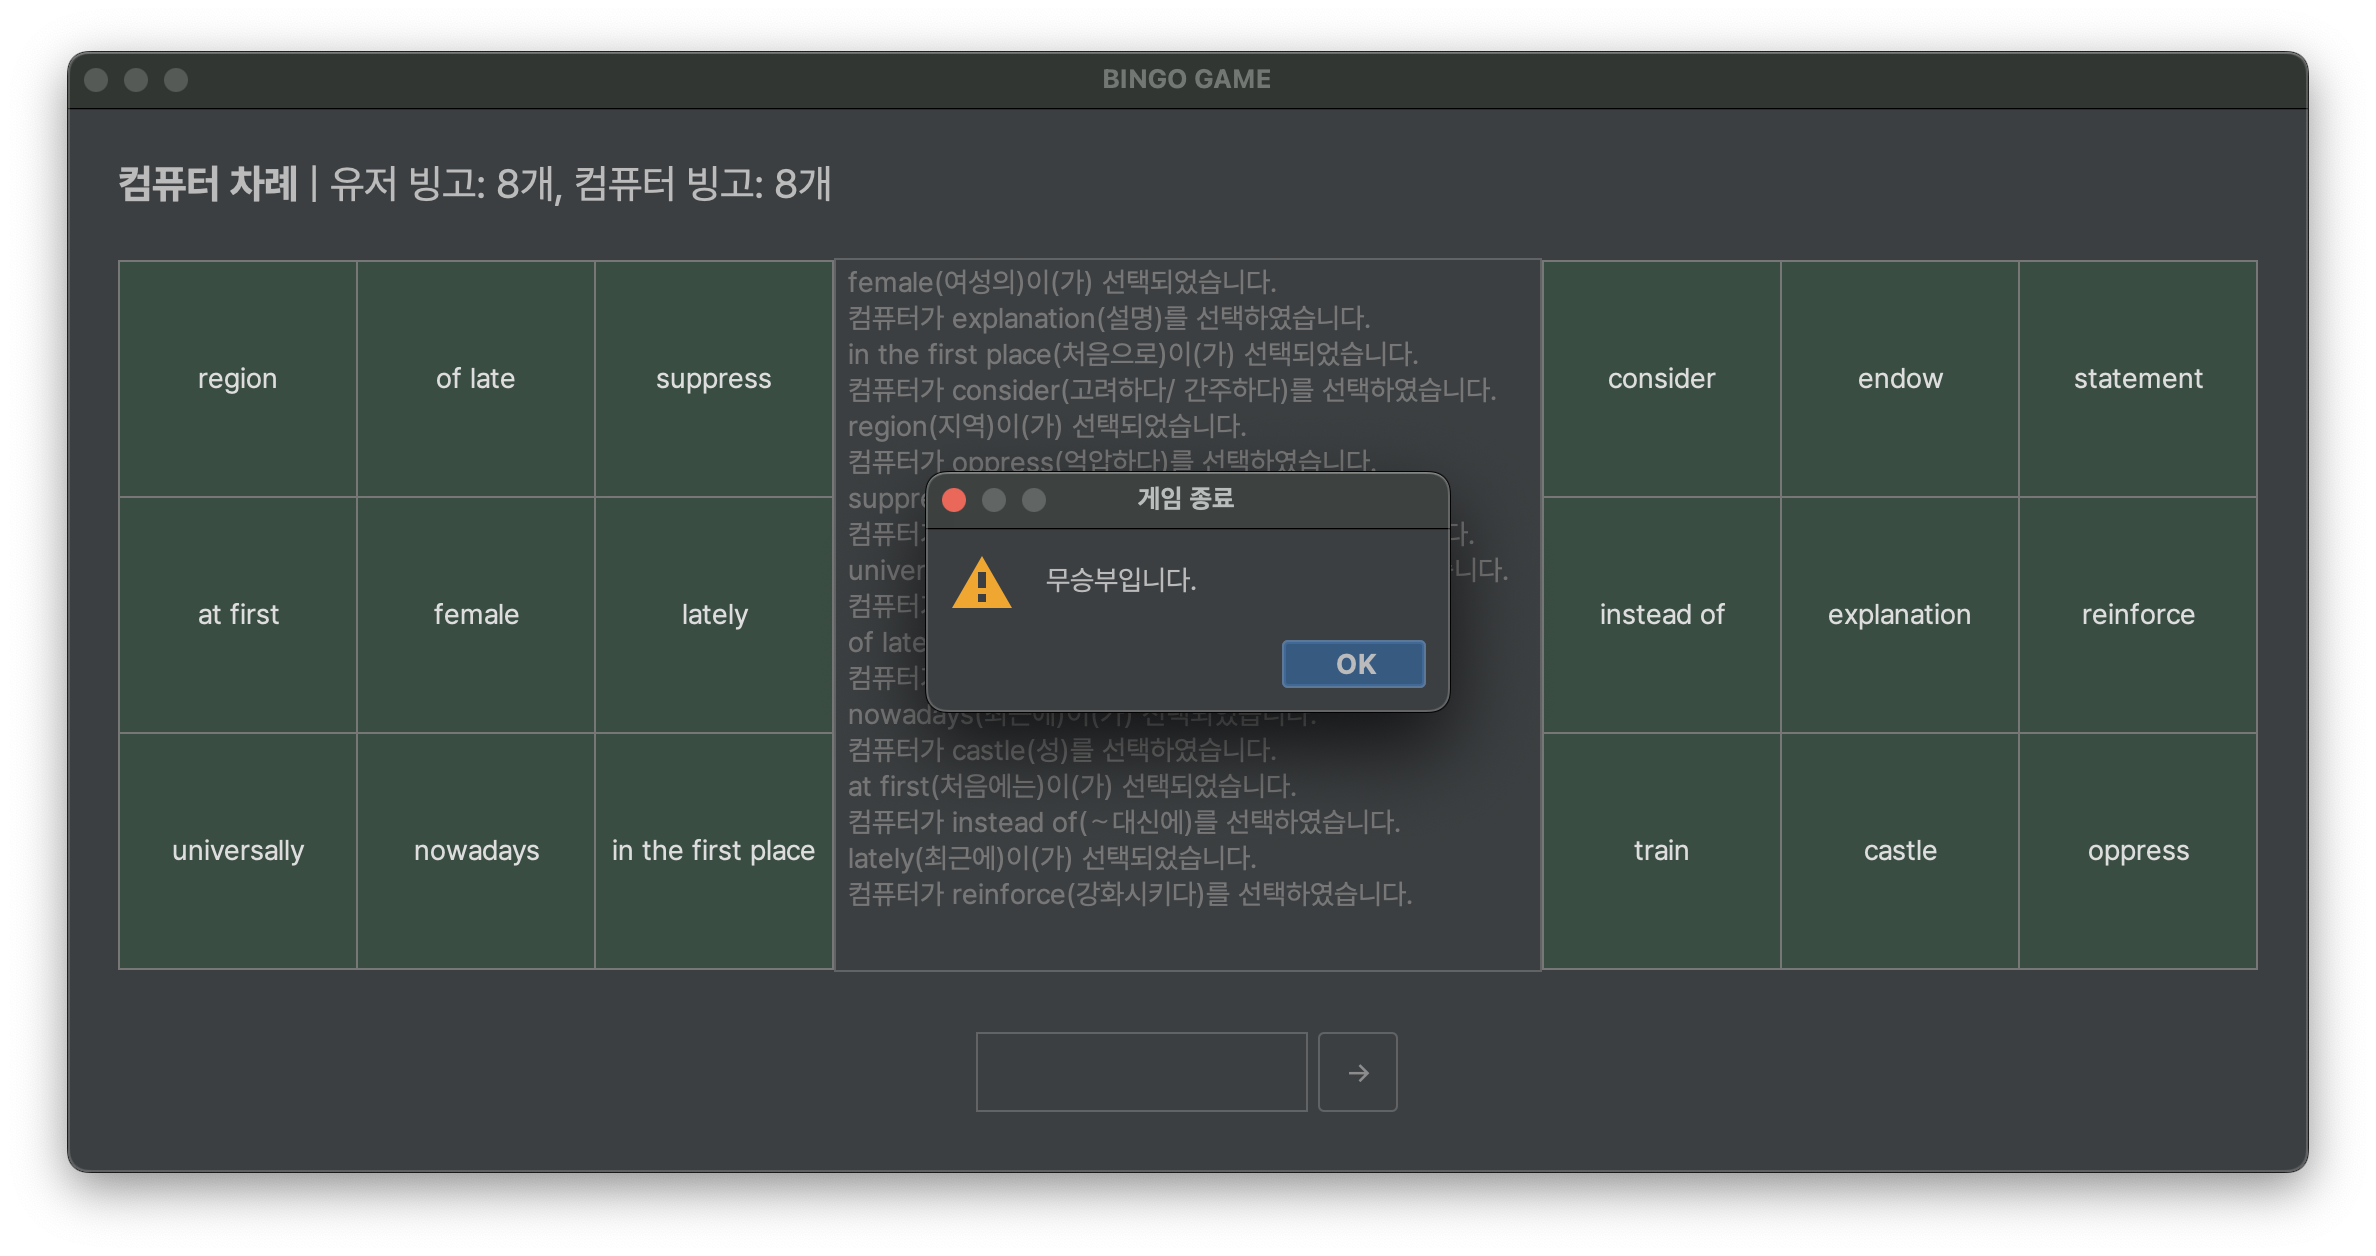
\includegraphics[scale=0.3]{img/game-3x3-draw.png}
        \caption{비겼을 때}
    \end{subfigure}
\end{figure}
\setcounter{figure}{6}
\begin{figure}[h]
    \begin{subfigure}{\textwidth}
        \centering
        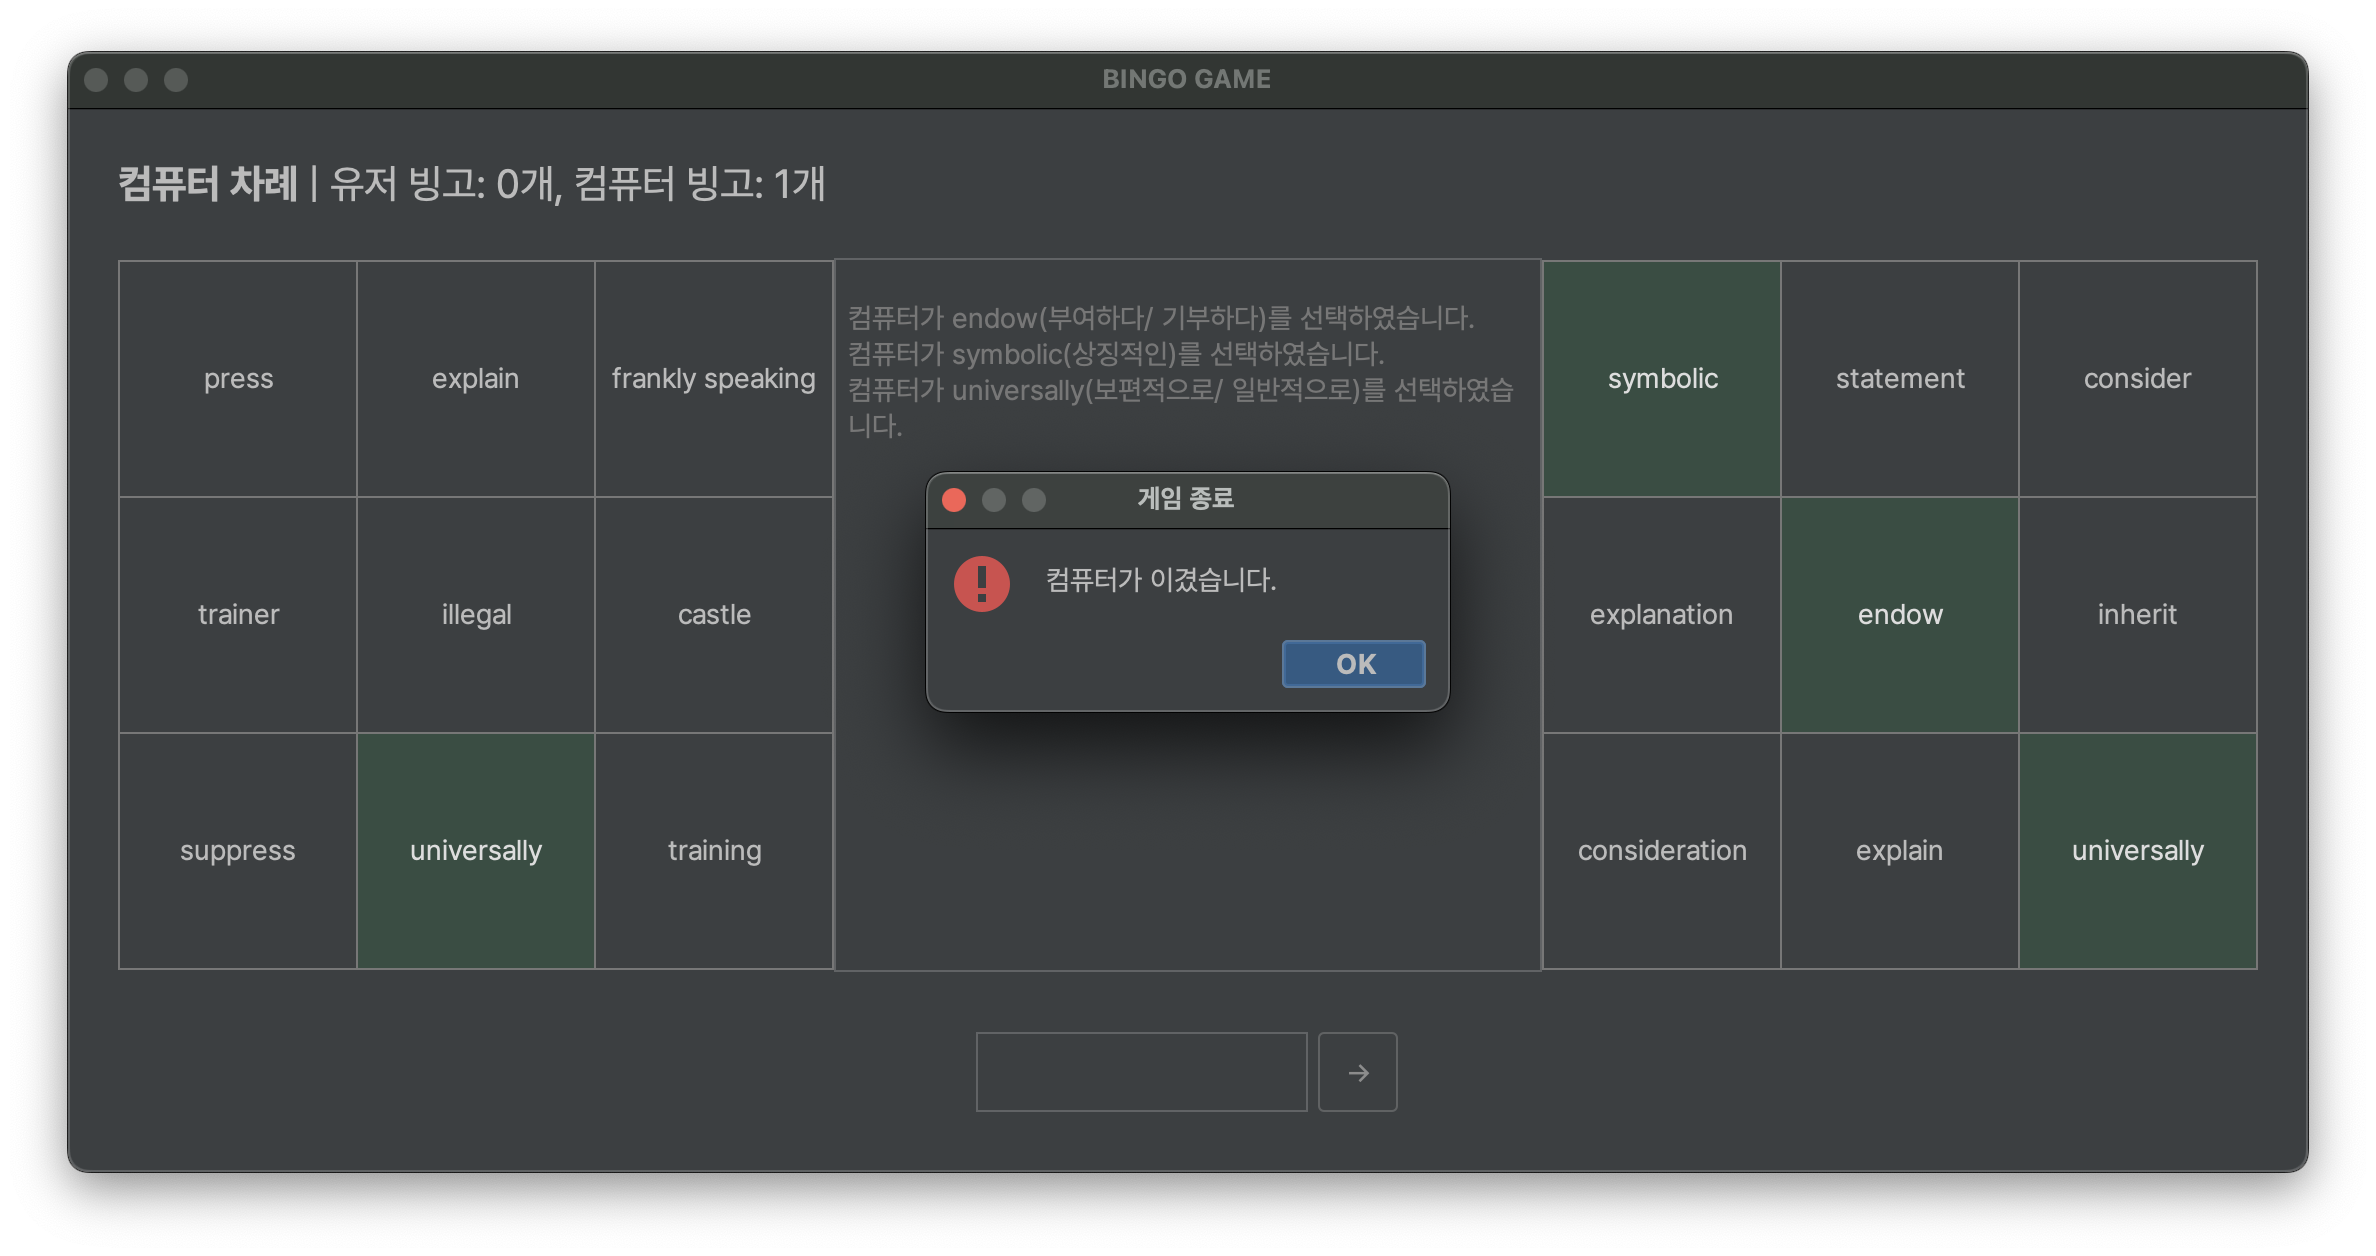
\includegraphics[scale=0.3]{img/game-3x3-defeat.png}\\
        (c) 졌을 때
    \end{subfigure}
    \caption{승패 처리 화면}
\end{figure}

\newpage
\begin{figure}[H]
    \begin{subfigure}{\textwidth}
        \centering
        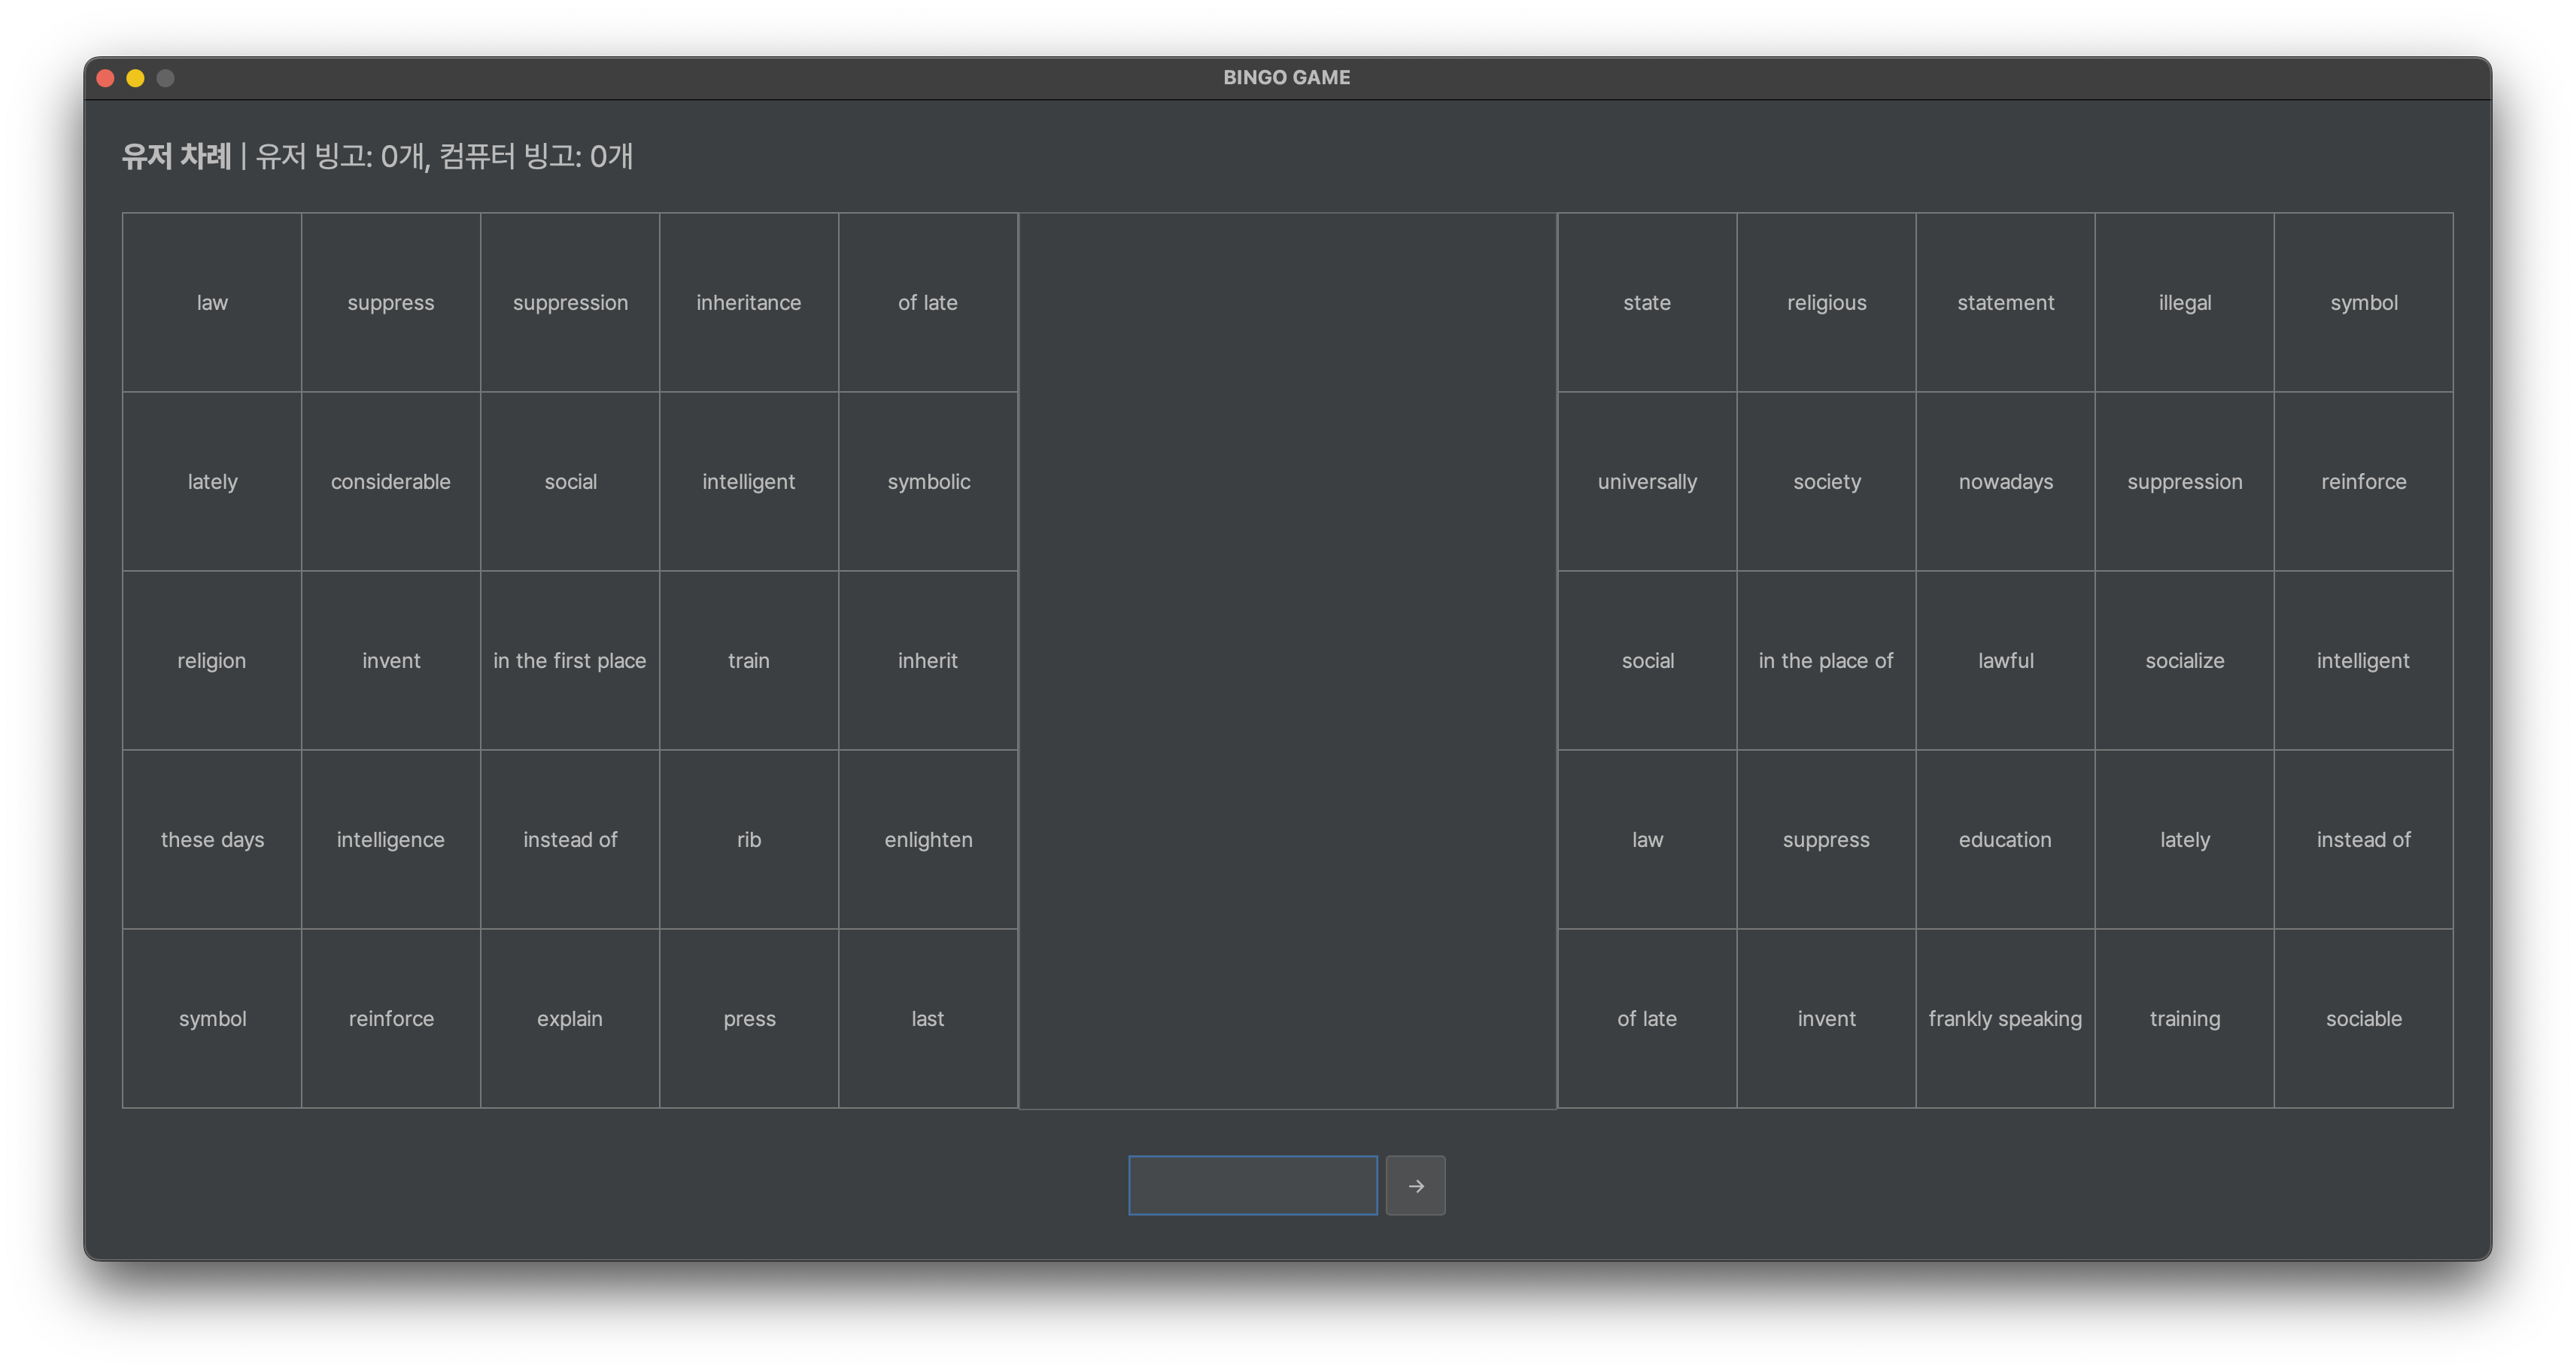
\includegraphics[width=0.9\textwidth]{img/game-5x5.png}
        \caption{$N = 5$}
    \end{subfigure}
\end{figure}
\newpage
\setcounter{figure}{7}
\begin{figure}[H]
    \begin{subfigure}{\textwidth}
        \centering
        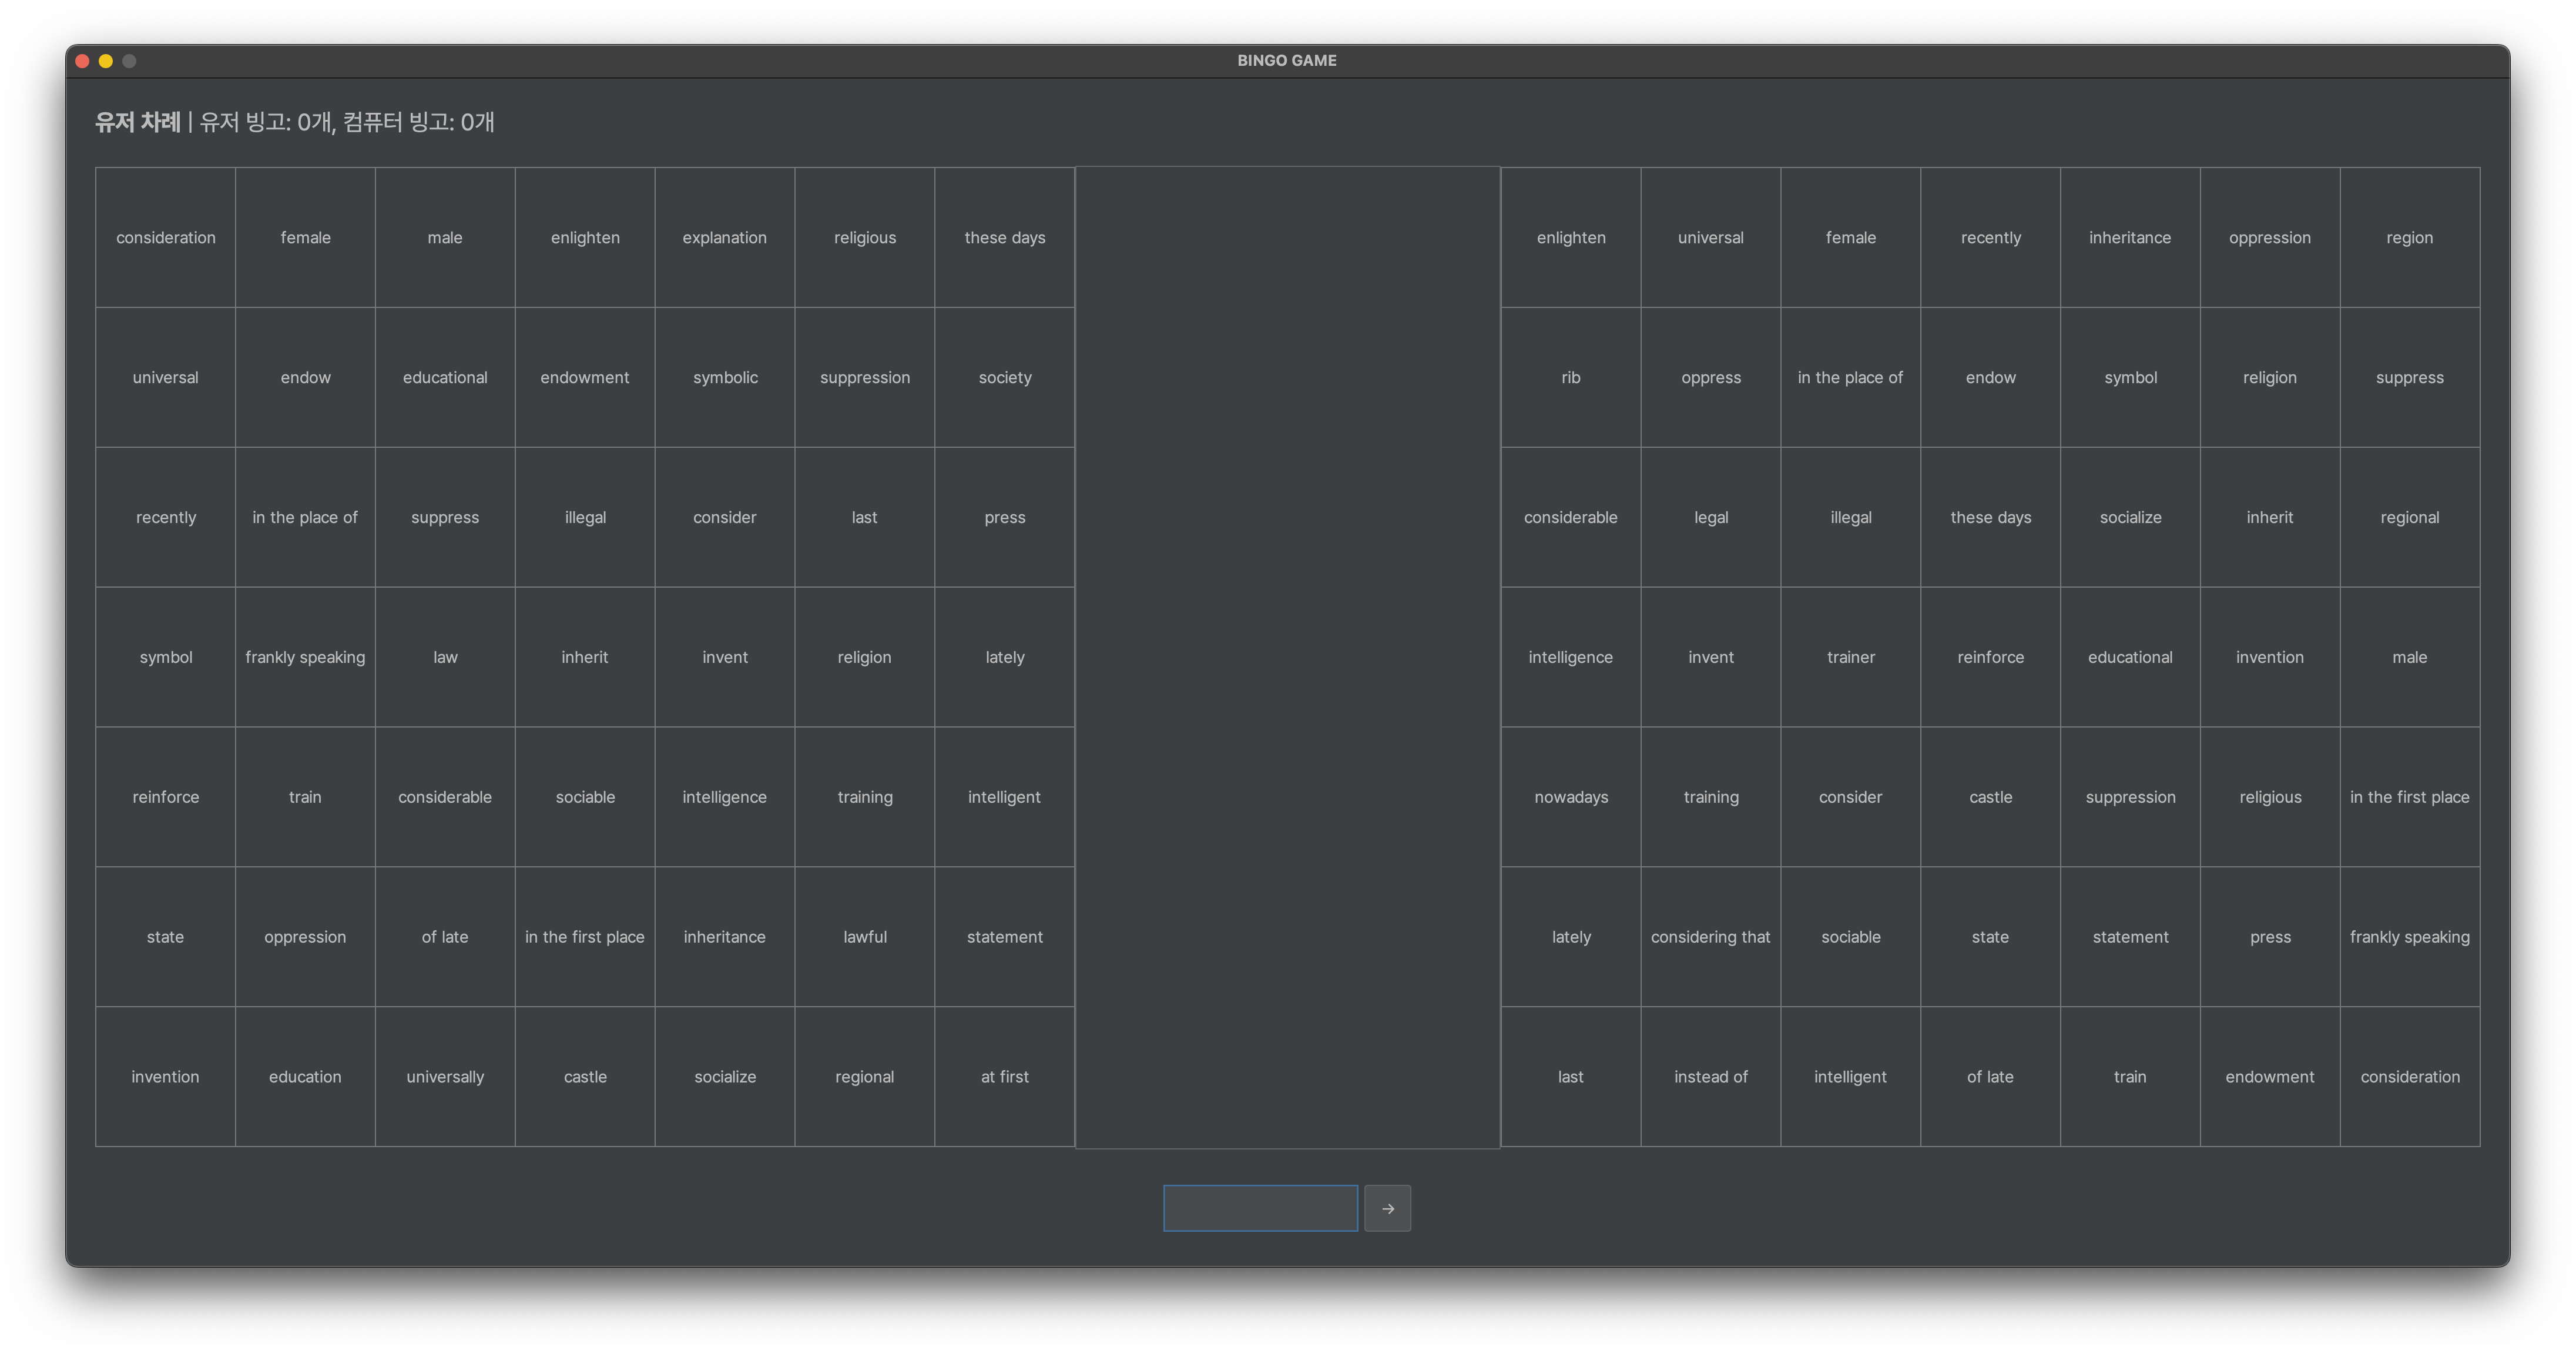
\includegraphics[width=0.9\textwidth]{img/game-7x7.png}\\
        (b) $N = 7$
    \end{subfigure}
    \caption{여러 크기의 $N$에 대한 빙고판}
\end{figure}
$3 \leq N \leq 10$ 사이의 모든 빙고판을 생성할 수 있다.

\newpage
\section{느낀점 및 토의 사항}
빙고 게임의 특성 상 유저와 컴퓨터 두 플레이어의 동일한 종류의 데이터를 다루어야 할 경우가 많기 때문에,
소스코드의 중복되는 부분을 줄이고, 가독성을 높이고자 적지 않은 수의 Class와 그에 딸린 함수들로 쪼개어 코드를 작성했다.
이로 인해 유지보수의 관점에서 봐도 추후 수정과 기능 추가에 유리할 것으로 판단된다.
또한 통계 기능에서, 여러 기능을 하는 함수들을 묶어 유틸리티 Class로 만들어 보는 등 이번 프로젝트를 진행하며 다양한 시도를 해보았다.

Swing으로 프로그램을 만들어 본 것이 처음이라 레이아웃을 짜는 데 어려움을 겪었지만,
원하는대로 레이아웃을 짜기 위해 여러 Layout들을 사용해보고, Java Documentation에서 Swing이 제공하는 Component들의 메소드를 찾아보는 과정에서 큰 도움이 된 것 같다.

팀 프로젝트로 진행하여 협업하며 코드를 작성하는 편이 더 재미있겠다고 생각해 개인적으로 이번 프로젝트가 개인 프로젝트로 진행된 점이 아쉬웠지만,
그만큼 여러 다양한 시도들도 해볼 수 있어서 역량 항상에는 큰 도움이 된 것 같았다.

\section{기타}
\subsection{개발 환경}
이 프로젝트를 개발하는 과정에서, 운영체제는 macOS 13.1 Ventura를 사용하였고, IDE는 Jetbrains사의 IntelliJ IDEA 2022.2.3 버전을 사용하였다.\\
JDK는 Temurin의 OpenJDK를 사용하였고, 버전 정보는 다음과 같다.\\
\texttt{
    openjdk 17.0.5 2022-10-18\\
    OpenJDK Runtime Environment Temurin-17.0.5+8 (build 17.0.5+8)\\
    OpenJDK 64-Bit Server VM Temurin-17.0.5+8 (build 17.0.5+8, mixed mode, sharing)
}

\subsection{참고 사항}
Swing의 UI 개선을 위해 오픈소스 라이브러리 Flatlaf(\url{https://github.com/JFormDesigner/FlatLaf})를 LookAndFeel로 적용하였다.
버튼 모양 등 수정하기 힘든 부분에서 UI의 개선을 이루고자 해당 라이브러리를 사용하였으며, 해당 라이브러리를 사용하지 않더라도 기능 면에서는 차이가 없기 때문에 최종 제출을 위한 소스코드에서는 주석 처리하였다. (BingoGame.jar의 12-22번 라인)

해당 라이브러리를 포함한 원본을 실행해보고자 한다면 첨부된 jar 파일을 더블 클릭하여 실행시키거나, 더블 클릭으로 실행되지 않을 경우 \texttt{java -jar} 명령어로 실행시키면 된다.

\subsection{수행 기간}
2022.11.28(월) - 2022.12.1(목)

\end{document}
